% Copyright 2004 by Till Tantau <tantau@users.sourceforge.net>.
%
% In principle, this file can be redistributed and/or modified under
% the terms of the GNU Public License, version 2.
%
% However, this file is supposed to be a template to be modified
% for your own needs. For this reason, if you use this file as a
% template and not specifically distribute it as part of a another
% package/program, I grant the extra permission to freely copy and
% modify this file as you see fit and even to delete this copyright
% notice. 

%\documentclass[handout]{beamer}
\documentclass[13pt]{beamer}

\title{On Bridging the Gap Between Theory and Practice in Statistical Learning}
\author{Andr\'as Gy\"orgy}
%Ruitong Huang$^1$ \and Tor Lattimore$^2$  \\ \medskip
%\textbf{$^3$} \and
%{Csaba Szepesv\'ari$^1$}}
%\\
%joint work with  and }
\institute{Department of Electrical and Electronic Engineering\\ Imperial College London}
\date{\tiny London, August 30, 2017 \\ \bigskip\bigskip
\small Based on joint work with Ruitong Huang, Csaba Szepesv\'ari, Tor Lattimore} % Lille



% If you have a file called "university-logo-filename.xxx", where xxx
% is a graphic format that can be processed by latex or pdflatex,
% resp., then you can add a logo as follows:

\titlegraphic{ 
%\includegraphics[height=10mm]{Imperial_2_Pantones.jpg} \hspace{5pt}
}

%\pgfdeclareimage[height=0.5cm]{university-logo}{logo}
%\logo{\pgfuseimage{university-logo}}

% There are many different themes available for Beamer. A comprehensive
% list with examples is given here:
% http://deic.uab.es/~iblanes/beamer_gallery/index_by_theme.html
% You can uncomment the themes below if you would like to use a different
% one:
%\usetheme{AnnArbor}
%\usetheme{Antibes}
%\usetheme{Bergen}
%\usetheme{Berkeley}
%\usetheme{Berlin}
\usetheme{Boadilla}
%\usetheme{boxes}
%\usetheme{CambridgeUS}
%\usetheme{Copenhagen}
%\usetheme{Darmstadt}
%\usetheme{default}
%\usetheme{Frankfurt}
%\usetheme{Goettingen}
%\usetheme{Hannover}
%\usetheme{Ilmenau}
%\usetheme{JuanLesPins}
%\usetheme{Luebeck}
%\usetheme{Madrid}
%\usetheme{Malmoe}
%\usetheme{Marburg}
%\usetheme{Montpellier}
%\usetheme{PaloAlto}
%\usetheme{Pittsburgh}
%\usetheme{Rochester}
%\usetheme{Singapore}
%\usetheme{Szeged}
%\usetheme{Warsaw}

%%%%%%% Author defined area %%%%%%%%%%%%

\usepackage[T1]{fontenc}
%\usepackage[latin9]{inputenc}

%%%%%%%%%%%%%% TODOs %%%%%%%%%%%%%%%%%%%%%%%%%%%%%
\usepackage{color}
%\usepackage[usenames,dvipsnames]{xcolor}


\setbeamerfont{frametitle}{size=\large}


\usepackage[absolute,overlay]{textpos}
%%%%
% note: beamer slides are 128mm by 96 mm
\newcommand{\putatUL}[4]{ % width xpos ypos WHAT; upper left corner is put at the said pos
\begin{textblock*}{#1}[0,0](#2,#3)
#4
 \end{textblock*}
}
\newcommand{\putatUR}[4]{ % width xpos ypos WHAT; upper right corner is put at the said pos
\begin{textblock*}{#1}[1,0](#2,#3)
#4
 \end{textblock*}
 }
\newcommand{\putatUM}[4]{ % width xpos ypos WHAT; upper right corner is put at the said pos
\begin{textblock*}{#1}[0.5,0](#2,#3)
#4
 \end{textblock*}
 }
\newcommand{\putatBR}[4]{ % width xpos ypos WHAT; bottom right corner is put at the said pos
\begin{textblock*}{#1}[1,1](#2,#3)
#4
 \end{textblock*}
}
\newcommand{\putatBL}[4]{ % width xpos ypos WHAT; bottom left corner is put at the said pos
\begin{textblock*}{#1}[0,1](#2,#3)
#4
 \end{textblock*}
}
\newcommand{\putatBM}[4]{ % width xpos ypos WHAT; bottom left corner is put at the said pos
\begin{textblock*}{#1}[0.5,1](#2,#3)
#4
 \end{textblock*}
}
 \newcommand{\putatMID}[4]{ % width xpos ypos WHAT; mid of image is put at the said pos
\begin{textblock*}{#1}[0.5,0.5](#2,#3)
#4
 \end{textblock*}
 }

\newcommand{\putat}[3]{\begin{picture}(0,0)(0,0)\put(#1,#2){#3}\end{picture}} % xrelpos yrelpos WHAT

\newcommand{\bcol}[1][t]{\begin{columns}[#1]} % optional argument: alignment (t,b,c)
\newcommand{\ecol}{\end{columns}}
\newcommand{\col}[1][0.5\textwidth]{\column{#1}} % argument: width of the column


%%%%%
\usepackage{tikz}
\usetikzlibrary{calc,shapes.callouts,shapes.arrows}

% Usage example:
% \arrowthis{There is}{Corot} a\speechthis{beautiful flower}{Van Gogh}\bubblethis{in}{Matisse}\pointthis{the garden}{Monet}.        
%
% From: http://tex.stackexchange.com/questions/38805/simple-speech-bubbles-arrows-or-balloon-like-shapes-in-beamer        

\newcommand{\arrowthis}[2]{
        \tikz[remember picture,baseline]{\node[anchor=base,inner sep=0,outer sep=0]%
        (#1) {{#1}};
        \node[overlay,single arrow,draw=none,fill=red!50,anchor=tip,rotate=60] 
        at (#1.south) {#2};}%
    }%

\newcommand{\speechthis}[2]{
        \tikz[remember picture,baseline]{\node[anchor=base,inner sep=0,outer sep=0]%
        (#1) {{#1}};\node[overlay,ellipse callout,fill=blue!50] 
        at ($(#1.north)+(-.5cm,0.8cm)$) {#2};}%
    }%

\newcommand{\bubblethis}[2]{
        \tikz[remember picture,baseline]{\node[anchor=base,inner sep=0,outer sep=0]%
        (#1) {{#1}};\node[overlay,cloud callout,callout relative pointer={(-0.6cm,-0.7cm)},%
        aspect=2.5,fill=yellow!90] at ($(#1.north)+(2.5cm,1.6cm)$) {#2};}%
    }%

\newcommand{\pointthis}[2]{
        \tikz[remember picture,baseline]{\node[anchor=base,inner sep=0,outer sep=0]%
        (#1) {{#1}};\node[overlay,rectangle callout,%
        callout relative pointer={(0.2cm,0.7cm)},fill=green!50] at ($(#1.north)+(-.5cm,-1.4cm)$) {#2};}%
        }%
        
\newcommand{\leftpointthis}[2]{
        \tikz[remember picture,baseline]{\node[anchor=base,inner sep=0,outer sep=0]%
        (#1) {{#1}};\node[overlay,rectangle callout,%
        callout relative pointer={(0.2cm,0.7cm)},fill=green!50] at ($(#1.north)+(-.5cm,-1.4cm)$) {#2};}%
        }%

\newcommand{\rightpointthis}[2]{
        \tikz[remember picture,baseline]{\node[anchor=base,inner sep=0,outer sep=0]%
        (#1) {{#1}};\node[overlay,rectangle callout,%
        callout relative pointer={(-0.3cm,0.7cm)},fill=green] at ($(#1.north)+(.5cm,-1.4cm)$) {#2};}%
        }%        
%%%%%%%        

\renewcommand<>{\cancel}[1]{\alt#2{\beameroriginal{\cancel}{#1}}{#1}}


\setbeamertemplate{navigation symbols}{}
\setbeamertemplate{footline}[frame number]
\setbeamercolor{math text}{fg=blue!50!normal text.fg}

\usepackage{multimedia}


% uncomment the following line and comment the line after it if you want to turn
% off todos
%\usepackage[textwidth=\marginparwidth]{todonotes}
\usepackage[disable,backgroundcolor = White,textwidth=\marginparwidth]{todonotes}
\newcommand{\todoc}[2][]{\todo[color=Apricot!20,size=\tiny,#1]{#2}}
\newcommand{\todot}[2][]{\todo[color=Cerulean!20,size=\tiny,#1]{#2}}
\newcommand{\todoa}[2][]{\todo[color=Purple!20,size=\tiny,#1]{#2}}
\newcommand{\todor}[2][]{\todo[color=Blue!10,size=\tiny,#1]{#2}}

\usepackage{xspace}
\usepackage{mathtools}
\usepackage{graphicx}
\usepackage[round]{natbib}
\usepackage{xspace}
\usepackage{multicol}
\newcommand\Fontvi{\fontsize{6}{7.2}\selectfont}

\usepackage{amsfonts}
\usepackage{amssymb}
\usepackage{amsmath}
\usepackage{amsthm}
\usepackage{mathtools}
\usepackage{verbatim}
\usepackage{epstopdf}
\usepackage{amstext}
%\usepackage{beamerthemesplit}
\usepackage{float}
%\usepackage{tipa}
\usepackage{fancyhdr}
\usepackage{rotating}
\usepackage{ulem}


\usepackage{esvect}

\allowdisplaybreaks
\newcommand{\cA}{\mathcal{A}}
\newcommand{\cB}{\mathcal{B}}
\newcommand{\cG}{\mathcal{G}}
\newcommand{\cX}{\mathcal{X}}
\newcommand{\cY}{\mathcal{Y}}
\newcommand{\cZ}{\mathcal{Z}}
\newcommand{\cW}{\mathcal{W}}
\newcommand{\cH}{\mathcal{H}}
\newcommand{\cF}{\mathcal{F}}
\newcommand{\cL}{\mathcal{L}}
\newcommand{\tcF}{\widetilde{\cF}}
\newcommand{\Exp}[1]{\mathbb{E}\left[ #1 \right]} 
\newcommand{\ind}{\mathbb{I}}
\newcommand{\one}[1]{\ind\left(#1\right)}
\newcommand{\seto}[1]{\left\{#1\right\}}
\newcommand{\real}{\mathbb{R}}
\newcommand{\R}{\mathbb{R}}
\newcommand{\bS}{\mathbb{S}}
\newcommand{\inpro}[2]{\langle #1, #2\rangle}
\newcommand{\inprol}[2]{\left\langle #1, #2\right\rangle}
\newcommand{\ip}[1]{\langle#1\rangle}
\newcommand{\set}[2]{\left\{#1 \,:\, #2 \right\}}
%\newcommand{\set}[2]{\left\{#1 \,\vert\, #2 \right\}}
\newcommand{\lt}{\ell_t}
\newcommand{\ttheta}{\tilde{\theta}}
\newcommand{\wtheta}{\widehat{\theta}}
\newcommand{\htheta}{\hat{\theta}}
\newcommand{\what}[1]{\widehat{#1}}
\newcommand{\tw}{\tilde{w}}
\newcommand{\hf}{\hat{f}}
\newcommand{\norm}[1]{\left\| #1 \right\|}
\newcommand{\bd}{\mathrm{bd}}
\newcommand{\inangle}[2]{(#1,#2)}
\newcommand\numberthis{\addtocounter{equation}{1}\tag{\theequation}}
\newcommand{\uD}{\overline{D}}
\newcommand{\lD}{\underline{D}}
\newcommand{\ra}{\rightarrow}
\newcommand{\eg}{\text{e.g. }}
\newcommand{\Prob}[1]{\mbox{Prob}\left(#1\right)}
\DeclareMathOperator*{\argmin}{argmin}
\DeclareMathOperator*{\argmax}{argmax}
\DeclareMathOperator{\dom}{dom}
\DeclareMathOperator{\epi}{epi}
\usepackage[capitalize]{cleveref}

%\newtheorem{thm}{Theorem}[section]
%\newtheorem{lemma}[thm]{Lemma}
%\newtheorem{prop}[thm]{Proposition}
%\newtheorem{cor}[thm]{Corollary}
%%\newtheorem{comm}[thm]{Comment}
%\newtheorem{example}[thm]{Example}
%\newtheorem{remark}[thm]{Remark}

\linespread{1.3}

%%%%%%%%%%%%%%%%%%%%%%%%%%%%%%%%%%%%%


%\setbeamertemplate{footline}{}
%\setbeamertemplate{navigation symbols}{}
% Delete this, if you do not want the table of contents to pop up at
% the beginning of each subsection:
%\AtBeginSection[]
%{
%  \begin{frame}<beamer>{Outline}
%    \tableofcontents[currentsection]
%  \end{frame}
%}

% Let's get started
\begin{document}

\begin{frame}
  \titlepage
\end{frame}

%\begin{frame}{Outline}
%  \tableofcontents
%  % You might wish to add the option [pausesections]
%\end{frame}

% Section and subsections will appear in the presentation overview
% and table of contents.

\newcommand{\bin}{\begin{itemize}}
\newcommand{\bi}{\begin{itemize}[<+->]}
\newcommand{\ei}{\end{itemize}}

\newcommand{\EEp}[1]{\mathbb{E}\left[#1\right]}
%\newcommand{\R}{\mathbb{R}}
%\newcommand{\norm}[1]{\|#1\|}
\newcommand{\snorm}[1]{\left\|#1\right\|} % scaling norm

\newcommand{\bc}{\begin{center}}
\newcommand{\ec}{\end{center}}
\newcommand{\eps}{\epsilon}
\newcommand{\nologo}{\setbeamertemplate{logo}{}} 
\newcommand{\ds}{$\diamondsuit$}


%%%%%%%%%%%%%%%%%%%%%%%%%%%%%%%%%%%%%%%%

\begin{frame}{Learning theory vs practice}
Statistical learning theory
\bin
\item Uses probabilistic models to analyze the trade-off between the amount of data and the achievable accuracy of learning for a given problem
\item The results are
\bin
\item brittle (what if the assumptions are not met)
\item can also be pessimistic as a result of focusing on obtaining worst-case guarantees
\ei
\ei
\pause
\bigskip
%\pause
Practice:
\bin
\item Learning algorithms often work outside of the scope of theoretical results
\item Examples:
\bin
\item Probabilistic/modeling assumptions are not met
\item Function classes are too large: (deep) neural networks, Gaussian processes, complicated models, etc.
\ei
\ei
\end{frame}

\begin{frame}{How to bridge the gap?}
\bi
\item Develop theory with little assumptions on the data generation (robustness)
\bi
\item e.g., online learning (adversarial, regret analysis of learning algorithms) \citep{CBLu06:book}\\ reinforcement learning with adversarial rewards (Neu, Gy, Szepesv\'ari, Antos, 2014; Dick, Gy, Szepesv\'ari, 2014)
\ei
\item Find properties that make the problem/data easy (invariance, hierarchy,  noise conditions, etc.)
\bi
\item e.g., "Easy data" workshops
\ei
\item Find maximal assumptions allowing to explain the observed performance
\ei
\end{frame}

\begin{frame}{How to bridge the gap?}
\bi
\item \alert{General strategy:} data-dependent analysis of algorithms by going beyond statistics
\begin{enumerate}[<+->]
\item Perform a deterministic analysis of the algorithm, reducing the problem to perturbation analysis
\item Perform statistical analysis on the size of perturbations when necessary or desired
\end{enumerate}
\ei



\bigskip
\pause
\begin{block}{}
In this talk: two examples when such an analysis is possible
\bi
\item unsupervised learning: independent component analysis
\item supervised learning: online learning (follow-the-leader algorithm)
\ei
\end{block}
\end{frame}

%Can we refine learning theory to bridge this gap? In this talk it will be demonstrated that this is possible in two quite different learning settings: One of the settings chosen is 
%an unsupervised problem (independent component analysis), the other is a supervised learning problem from online learning. For both problems, results will be given that explain in detail various earlier observed gaps between theory and practice. The broader claim is that with the approach presented, learning theory can successfully contribute beyond its usual boundaries, by providing refined performance bounds with little or no assumptions on data generation and eventually leading to better algorithms for a wide range of learning settings.
%\end{frame}

%\section{Introduction}
%\subsection{What is ICA, really?} %{What is ICA, really? A little bit of philosophy for machine learning theorists}

\frame{
\centering
\color{blue}{
\Huge Example 1: Deterministic Independent Component Analysis
}}

\frame{ \frametitle{What is Independent Component Analysis (ICA)?}

\bc
\includegraphics[height=0.9\textheight]{ICABookCover}
\ec

%\includegraphics{Aapo}
%\begin{block}{}
%Independent component analysis (ICA) is a statistical and computational technique for revealing hidden factors that underlie sets of random variables, measurements, or signals.
%\end{block}
}

\frame{
\includegraphics{ICABOOK2001_ObservedSignals}
\vspace*{-0.1in}
\bc
$x(t)=As(t),t\in [T]:= \{1,\dots,T\}$
\ec
}

\frame{
\includegraphics{ICABOOK2001_ReconstructedSignals}
}

\begin{frame}{}
\begin{block}{}
\bc
\includegraphics[width=0.3\textwidth]{ICABOOK2001_ObservedSignals}
\hspace{0.1\textwidth}\includegraphics[width=0.3\textwidth]{ICABOOK2001_ReconstructedSignals}
\ec
\end{block}
\vspace*{-0.05in}
{\linespread{1.2} \small 
\begin{quotation}
\uncover<+->{%
``Using just this information on the \alert{statistical independence}, we can in fact estimate the coefficient matrix \sout{$W$} $A$ for the signals in Fig. 1.2. 
}
\uncover<+->{%
What we obtain are the source signals in Fig. 1.3. (These signals were estimated by the FastICA algorithm [...].)} % that we shall meet in several chapters of this book.)}
\uncover<+->{%
We see that from a data set that seemed to be just noise, we were able to estimate the original source signals, using an algorithm that used the information on the \alert{independence only}.
}
\uncover<+->{%
These estimated signals are indeed equal to those that were used in creating the mixtures in Fig. 1.2 
(the original signals are not shown, but they really are virtually identical to what the algorithm found). 
}
\uncover<+->{%
Thus, in the source separation problem, the original signals were the ``independent components'' of the data set.''}
\end{quotation}
}
\end{frame}

\begin{frame}{}
\begin{block}{}
\bc
\includegraphics[width=0.3\textwidth]{ICABOOK2001_ObservedSignals}
\hspace{0.1\textwidth}\includegraphics[width=0.3\textwidth]{ICABOOK2001_ReconstructedSignals}
\ec
\end{block}
\vspace*{-0.05in}
{\linespread{1.2} \small 
\begin{quotation}
\uncover<+->{This leads us to the following definition of ICA [$\dots$]}
\uncover<+->{Given a set of observations of random variables
$(x_1(t),x_2(t),\dots,x_d(t))$, 
where $t$ is the time or sample index, 
assume that they are generated as a linear mixture of \alert{independent components}:}
\uncover<+->{
\[
\begin{pmatrix}
x_1(t)\\x_2(t)\\ \vdots \\ x_d(t)
\end{pmatrix} = A
\begin{pmatrix}
s_1(t)\\s_2(t)\\ \vdots \\ s_d(t)
\end{pmatrix}\,,
\]
where $A$ is some unknown matrix.}
\uncover<+->{%
Independent component analysis now consists of estimating both the matrix $A$ and the $s_i(t)$, when we only observe the $x_i(t)$.}
\end{quotation}
}

%\vspace{-7.2cm}
%\pause
%\begin{center}
%\begin{minipage}{0.5\textwidth}
%\begin{alertblock}{}\begin{center}\medskip \Huge Looks good? \medskip\end{center}\end{alertblock}
%\end{minipage}
%\end{center}
%\vspace{7.2cm}
%
\end{frame}


\frame{
\frametitle{Independence?}

\vspace*{-0.45in}
\mbox{}\hspace*{0.5\textwidth}
\begin{minipage}{0.45\textwidth}
\begin{block}{}
\includegraphics[width=0.95\textwidth]{ICABOOK2001_ReconstructedSignals}
\end{block}
\end{minipage}

\bi
\item Is $s_1(t)$ independent of $s_2(t)$? \uncover<+->{Of course!} \uncover<+->{How about $s_1(t)$ and $s_3(t)$?}
\item Any two numbers are independent of each other! 
\uncover<+->{All deterministic signal sources are fine then?}
\item Should we be worried about temporal dependencies? %\uncover<+->{No?}
\uncover<+->{What if $s_1(t) = s_1(t+1) = \dots$? }
\item What is ICA then???
%\item Leon Bottou (ICML 2015): \alert{Can't reduce everything to statistics!}
%\item Here: \alert{Let's go beyond statistics!}
\ei
}


%\subsection{Deterministic ICA}
%\begin{frame}{Outline}
%\tableofcontents[currentsection,currentsubsection]
%\end{frame}

\linespread{1.2}


\frame{
\frametitle{What signals can be separated?}
\small
\bi
\item \uncover<+->{Wrong question!}
\item Better: To what extent can we separate the mixture of some signals?
\ei

\uncover<+->{
Let $[T] = \{1,\dots,T\}$.
Sources:  $s:[T] \to [-C,C]^d$.
}

\uncover<+->{
Let $\nu_T^{(s)}$ be the empirical distribution induced by $s$; for $B\subset [-C,C]^d$,
	\[
	\nu_T^{(s)}(B)=\tfrac{1}{T}|\{t \in [T]: s(\tau) \in B\}|.
	\]
}

\begin{block}<+->{Measure of independence}
%Our independence measure:
	\[
	D_4	= \inf_{\mu} \sup_{f\in\mathcal{F}} \Big|\int f(s)d\nu_T^{(s)} - \int f(s)d\mu(s)\Big|,
	\]
 $\mathcal{F}$: the set of all monomials up to degree $4$;\\
  $\mu$: any product measure.
\end{block}


\uncover<+->{
\textcolor{blue}{Note}:
When $s(t)$ has independent components and $s(1),\dots,s(T)$ are iid,
$D_4 = O(1/\sqrt{T})$.
}
}

\if0
\frame{ \frametitle{Independent Component Analysis (ICA)} 
\bi 
%\item A special case of Blind Source (Signal) Separation;
\onslide<+->
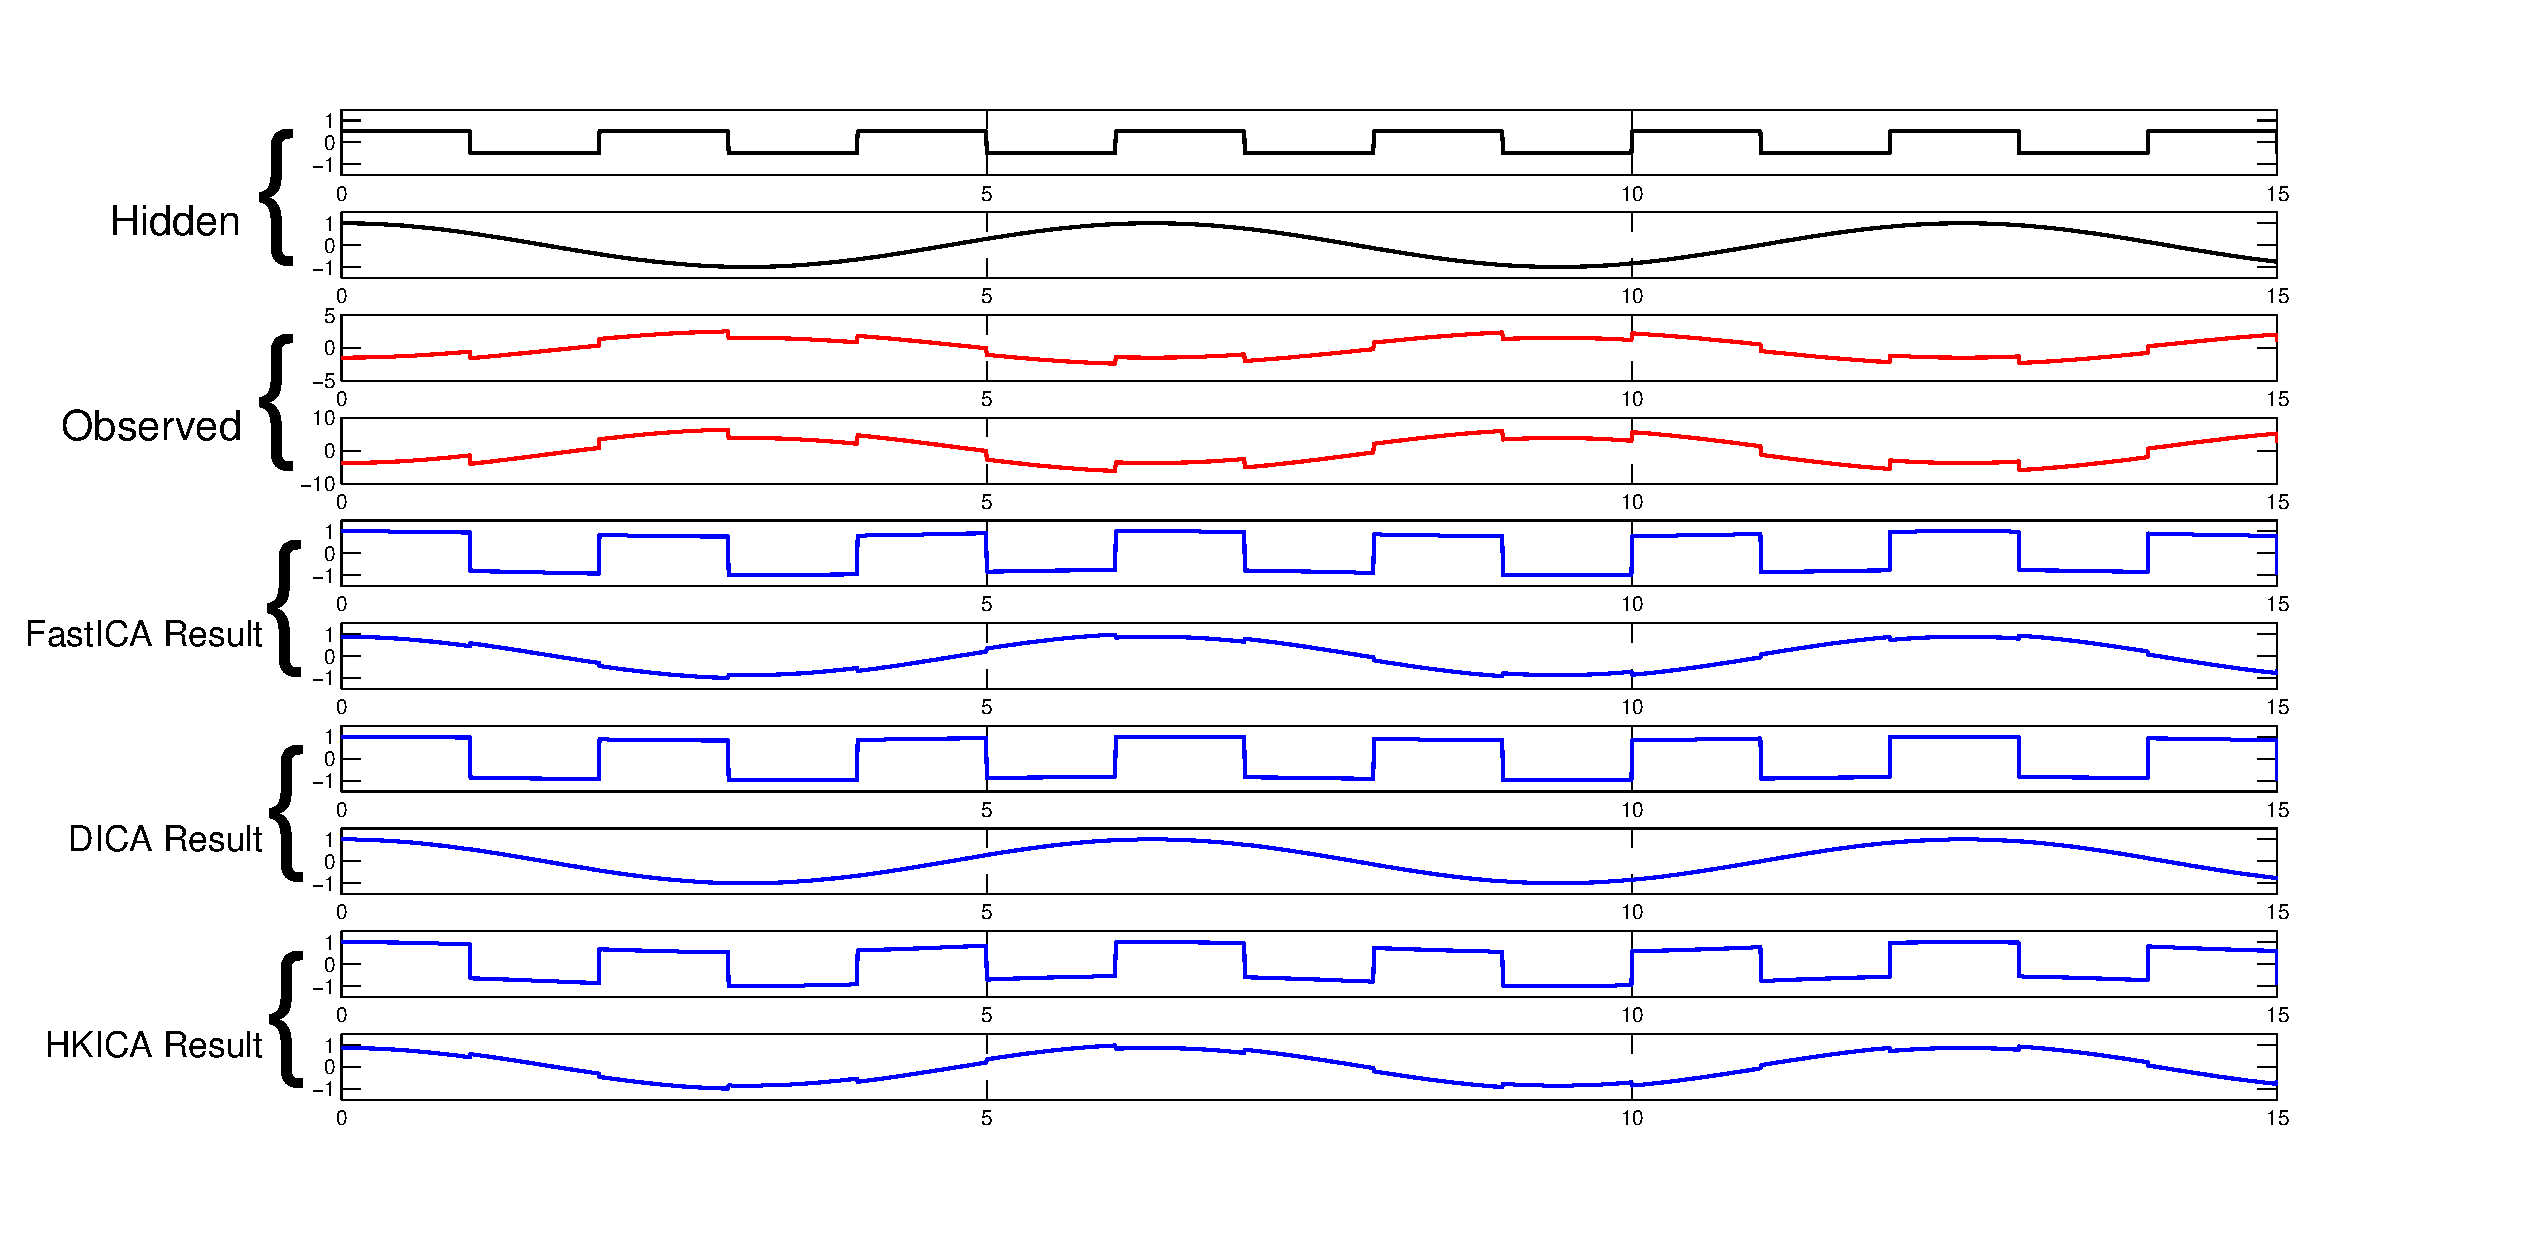
\includegraphics[width=.9\textwidth]{demo}
\ei
}
\fi

\if0
\frame{ \frametitle{Independent Component Analysis (ICA)} 
\bi 
\item  Model: $X = AS + \epsilon$; \\
\onslide<+->
\begin{center}
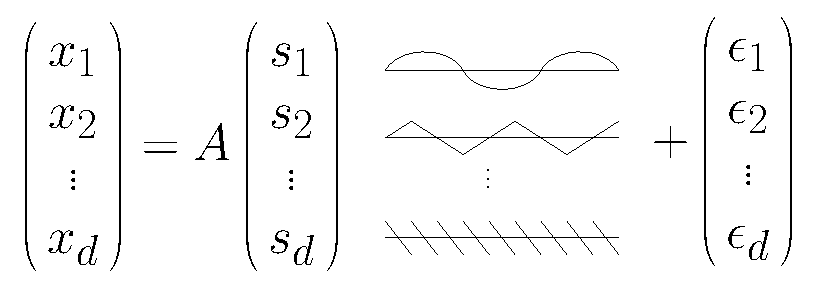
\includegraphics[width=8cm]{ICA_model.eps}
\end{center}
\item $S = (S_1,\ldots, S_d)$ non-Gaussian, $\eps \sim \mathcal{N}(0,\Sigma)$ Gaussian random variables.
\item Goal: Given $T$ independent observations $X(1), \ldots, X(T) \sim X$, reconstruct $A$ up to scaling and permutation. 
\ei
}
\frame{ \frametitle{Independent Component Analysis (ICA)} 
\begin{center}
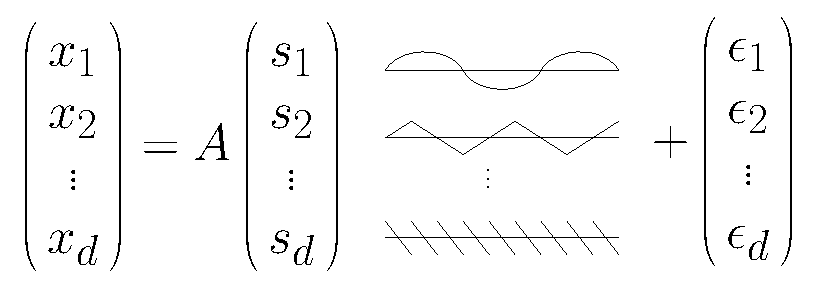
\includegraphics[width=8cm]{ICA_model.eps}
\end{center}
\bi
\item Assumptions:
	\bi
	\item[--] $S_1(t),\ldots, S_d(t)$, $\eps_1(t), \ldots, \eps_d(t)$ are mutually independent for any $t$.
	\vspace{0.3cm}
	\item[--] $A$ is non-singular (for simplicity). 
	\ei
\item Applications: Optical imaging; Telecommunications; Biology; Medicine. 
\ei
}
\fi

\frame{
\frametitle{Goal}
Assuming $x(t) = A s(t) + \eps(t)$, $t=1,\dots, T$;
\\ $\eps(t)$ ``noise''.\\

\medskip

Can we find a method with the following characteristics?

\bi
\setlength{\itemsep}{10pt}
\item Universal: No free parameters!
\item Efficient:  $\mathrm{poly}(T,d)$ runtime (no dependence on $C$, $A$, $\dots$);
\item Robust \& noise-tolerant: $\mathrm{lin}(D_4+1/\sqrt{T})$ accurate in recovering $A$ (with i.i.d. observation noise)?
\ei

\uncover<+->{
Accuracy measure:
\[
d(\hat{A},A) = \inf_{
	 \substack{\pi \in \mathrm{Perm}([d])\\
	 c\in \R^d}} \max_{k} 
	|| c_k \hat{A}_{:\pi(k)} - A_{:k} ||_2\,.
\]
}
}

%\subsection{Has not this been done previously?}
%\begin{frame}{Outline}
%\tableofcontents[currentsection,currentsubsection]
%\end{frame}

\frame{ 
\frametitle{Previous works with theoretical guarantees} 

\onslide<+->
\citet{SaTsy04,CheBi06} and others: 
\bi
\item No noise
\item Semi-parametrics, ``average derivative estimation'';
\item Asymptotics: $\sqrt{n}$ consistency and efficiency;
%\item Why estimate something that is then thrown away? (Also: We'll need conditions on these$\dots$)
\ei
\medskip

\onslide<+->
FastICA by \citet{hyvarinen1999fast}:
\bi
\item Perhaps the most popular ICA algorithm.
\item With probability 1, all local optimizers are desired solutions \citep{wei2014study}, given:
	\begin{itemize}
	\item[--]<2-> infinitely many noiseless samples;
	\item[--]<2-> using kurtosis as the scoring function.
	\end{itemize}
\item[-] Weakness: noisy periodic signals;
\ei

\onslide<+->
%\vspace{1cm}
Moment methods: \citep{frieze1996learning,DHsu2012, arora2012provable,goyal2014fourier}.
}

\frame{ \frametitle{Moment methods}
\bi
\item \citet{frieze1996learning}: 
\bi
\item[-] No noise allowed (also: minor gap fixed by \citet{arora2012provable});
\ei
\item \citet{DHsu2012} (``HKICA''):
\bi
\item[-] No theoretical guarantee stated;
\item[-] If we do the analysis, accuracy will depend on $\gamma_A$; an uncontrolled parameter (see later).
\ei
\item \citet{arora2012provable}:
\bi
\item[-] Free parameter ``$\beta$'', whose choice depends on $||A_{:i}||_2$, while $x\in \{-1,+1\}^d$.
\item[-] Choose either the scale of sources or the scale of the columns of $A$, not both!
\ei
\item Fourier PCA \citep{goyal2014fourier} (FPCA):
\bi
\item[-] Free parameter: Same problem as with \citet{arora2012provable}'s approach.
\ei
%\\
%\quad - If you assume that both the mixing matrix and the sources are bounded with a known bound, 
%the parameter can be chosen.
%\\
\ei

\uncover<+->{\centering \alert{Why care about a free parameters?}}
\uncover<+->{\centering $\dots$ \textcolor{blue}{unsupervised} learning}
%This is unsupervised learning!\\
%Cross-validation is messy at best.
%\end{block}
}


%\section{Results}
%\subsection{Main result}
%\begin{frame}{Outline}
%\tableofcontents[currentsection]
%\end{frame}

\frame{ \frametitle{Main Result}
There exist a randomized algorithm DICA that maps $(x(t))_{t=1}^T\in \R^{d\times T}$ to $\hat{A}\in \R^{d\times d}$ such that
for all $(x,s,A)$, $x(t)=A s(t) + \eps(t)$, $t=1,\dots,T$,
\medskip
\bi
\setlength\itemsep{1em}
\item the computational complexity of DICA is $O(d^3 T)$;
\item with high probability, the output $\hat{A}$ satisfies
	\[
	d(\hat{A},A) \le \theta_1 \min( D_4(s) + 1/\sqrt{T}, \theta_2 )\,,
	\]
%\item[] 
where $\theta_1,\theta_2$ are problem-dependent, polynomial in the ``parameters'' (scales, conditioning, kurtosis).
\ei
}


%\subsection{The DICA (Deterministic ICA) Algorithm}
%\begin{frame}{Outline}
%\tableofcontents[currentsection]
%\end{frame}


\frame{ \frametitle{Hsu-Kakade method (HKICA)} 
\uncover<+->{For $x=As$, $s\sim \mu=\mu_1\otimes \dots \otimes \mu_d$,
$\eta \in \R^d$, let 
%\vspace*{-0.15in}
\[
f(\eta) = \EEp{(\eta^{\top}x)^4} - 3 \EEp{(\eta^{\top}x)^2}^2\,.
\]}
\vspace*{-0.35in}
\begin{columns}[t]
\column{0.5\textwidth}
\bi
\item[-] Choose $\phi$ and $\psi$. \emph{(How?)}
\item[-] Let $T(\phi) = \nabla^2 f(\phi)$. Then 
\[T(\phi) = AK 
\left(
\begin{array}{ccc}
\sigma_1 & & \\ 
    & \ddots & \\
    & & \sigma_d
\end{array} 
\right) 
A^{\top},
\]
where $\sigma_i = \left(\phi^{\top}A_i\right)^2$ and $K$ is some diagonal matrix.
\item[-] Let $M = T(\phi)(T(\psi))^{-1}$.
\ei
\column{0.5\textwidth}
\bi
\item[-] Then 
\[M = A 
\left(
\begin{array}{ccc}
\lambda_1 & & \\ %\left(\frac{\phi^{\top}A_1}{\psi^{\top}A_1}\right)^2 & &\\
    & \ddots & \\
    & & \lambda_d %\left(\frac{\phi^{\top}A_d}{\psi^{\top}A_d}\right)^2\\
\end{array} 
\right) 
A^{-1},
\]
where $\lambda_i = \left(\frac{\phi^{\top}A_i}{\psi^{\top}A_i}\right)^2$.
\item[-] Do an eigen-decomposition of $M$ to recover $A$, assuming all $\lambda_i$'s are distinct.
%\item[-] 
\ei
\end{columns}
\medskip
\uncover<+->{
\centering
Given finite sample $(x(t))_{t=1}^T$, replace $\mathbb{E}[\cdot]$ with $\mathbb{E}_T[\cdot]$.}
}

\if0
\frame{ \frametitle{Hsu-Kakade method (HKICA)} 
\bi
\item[-] Let $M = T(\phi)(T(\psi))^{-1}$. Then 
\[M = A 
\left(
\begin{array}{ccc}
\lambda_1 & & \\ %\left(\frac{\phi^{\top}A_1}{\psi^{\top}A_1}\right)^2 & &\\
    & \ddots & \\
    & & \lambda_d %\left(\frac{\phi^{\top}A_d}{\psi^{\top}A_d}\right)^2\\
\end{array} 
\right) 
A^{-1},
\]
where $\lambda_i = \left(\frac{\phi^{\top}A_i}{\psi^{\top}A_i}\right)^2$.
\item[-] Do an eigen-decomposition of $M$ to recover $A$, assuming all $\lambda_i$'s are distinct.
\item[-] Given $(x(t))_{t=1}^T$, replace $\EE{\cdot}$ with $\mathbb{E}_n{\cdot}$.
\ei
}
\fi

\frame{ \frametitle{The issue with the HK method}
{\large{Problem: Minimal gap of the eigenvalues.}}			
\bi
\item Theoretical analysis shows that the performance depends on $\gamma_A^{-1}$, where
	\[
	\gamma_A = \min_{i\neq j} \left\vert \lambda_i - \lambda_j\right \vert.
	\]
\item $\gamma_A$ is not  well understood%
\footnote{Is $\gamma_A^{-1}$ polynomially bounded in $d$?}
%\item[] in particular, it is not known whether $\gamma_A^{-1} = \mathrm{Poly}(d,A)$\,.
\ei
\bigskip

\uncover<+->{
\centering 
\Large 
\alert{Goal}: Avoid dependency on $\gamma_A^{-1}$!
}
}

\frame{ \frametitle{Our method: Deterministic ICA (DICA)}
\bi
\item[--] Inspired by \citet{arora2012provable} and \citet{frieze1996learning};
\item[--] Sample $\psi$, $\phi_1$ and $\phi_2$ independently from standard normal distribution.
\item[--] Calculate $\nabla^2 f(\psi)$ and $B$ such that $\nabla^2 f(\psi) = BB^{\top}$.%
\bi
\item Recall: $f(\eta) = \EEp{(\eta^{\top}x)^4} - 3 \EEp{(\eta^{\top}x)^2}^2$
\ei
\item[--] Calculate $T(\phi_1) = \nabla^2 f(B^{-\top}\phi_1)$ and $T(\phi_2) = \nabla^2 f(B^{-\top}\phi_2)$.
\item[--] Calculate $M = T(\phi_1)(T(\phi_2))^{-1}$. Note:
	\[
	M = R \,\mathrm{diag}\left( \tilde{\lambda}_1, \ldots, \tilde{\lambda}_d \right)R^{\top},
	\]
	where $\tilde{\lambda}_i = \left(\frac{\phi_1^{\top}R_i}{\phi_2^{\top}R_i}\right)^2$ and $R$ is some \alert{orthonormal} matrix
	s.t. \alert{$A = BR$}.
\item[--] Do an eigen-decomposition of $M$ to recover $R$.
\item[--] Return $\hat{A} = BR$ as an estimate of $A$. 
\ei
}

\frame{ \frametitle{Our method: Deterministic ICA (DICA)}
\bi
\item The reconstruction error is proportional to $\gamma_R^{-1}$, where 
	\[ 
	\gamma_R = \min_{i\neq j} \left\vert \tilde{\lambda}_i - \tilde{\lambda}_j\right \vert = \min_{i\neq j} \left\vert \left(\frac{\phi_1^{\top}R_i}{\phi_2^{\top}R_i}\right)^2
	 - \left(\frac{\phi_1^{\top}R_j}{\phi_2^{\top}R_j}\right)^2\right\vert.
	\]
	\bi
	\item[--] $\{\phi_1^{\top}R_1,\ldots, \phi_1^{\top}R_d, \phi_2^{\top}R_1,\ldots, \phi_2^{\top}R_d \}$ are independent standard normal variables.
	\item[--] No dependency on $A$.
	\item[--] Can be reduced to the minimal spacing of Cauchy random variables.
	\ei
\item Recursive version is also developed in the paper, based on the idea of \citet{vempala2014max}.
\ei
}

%\section{Empirical Illustration}
%\begin{frame}{Outline}
%\tableofcontents[currentsection]
%\end{frame}

\frame{ \frametitle{Setting}
\begin{columns}[t]
\column{0.5\textwidth}
\uncover<+->{Questions:}
\bi
	\item Does noise matter?
		\bi
		\item[-] Additive Gaussian noise.
		\ei
	\item Does coherence matter? 
		\bi 
		\item[-] $R, A_1, A_2, A_3, A_4$: Gaussian matrices with increasing coherence.
		\ei
	\item Do the recursive versions improve the results?
\ei
\column{0.5\textwidth}
\uncover<+->{Algorithms:}
\bin
	\item FastICA  \citep{szabo14information} %\citep{szabo12separation};
	\item HKICA/HKICA.R; 
	\item (recursive) FPCA due to \citet{vempala2014max};
%	\item<1-> Random guessing (Random).
	\\ \mbox{}\\
	\item DICA/DICA.R; 
	\item MDICA/MDICA.R (heuristic version of DICA)
\ei
\end{columns}

}

\frame{
\frametitle{Sources}

BPSK (binary phase-shift keying) sources, $T=20,000$:
\bc
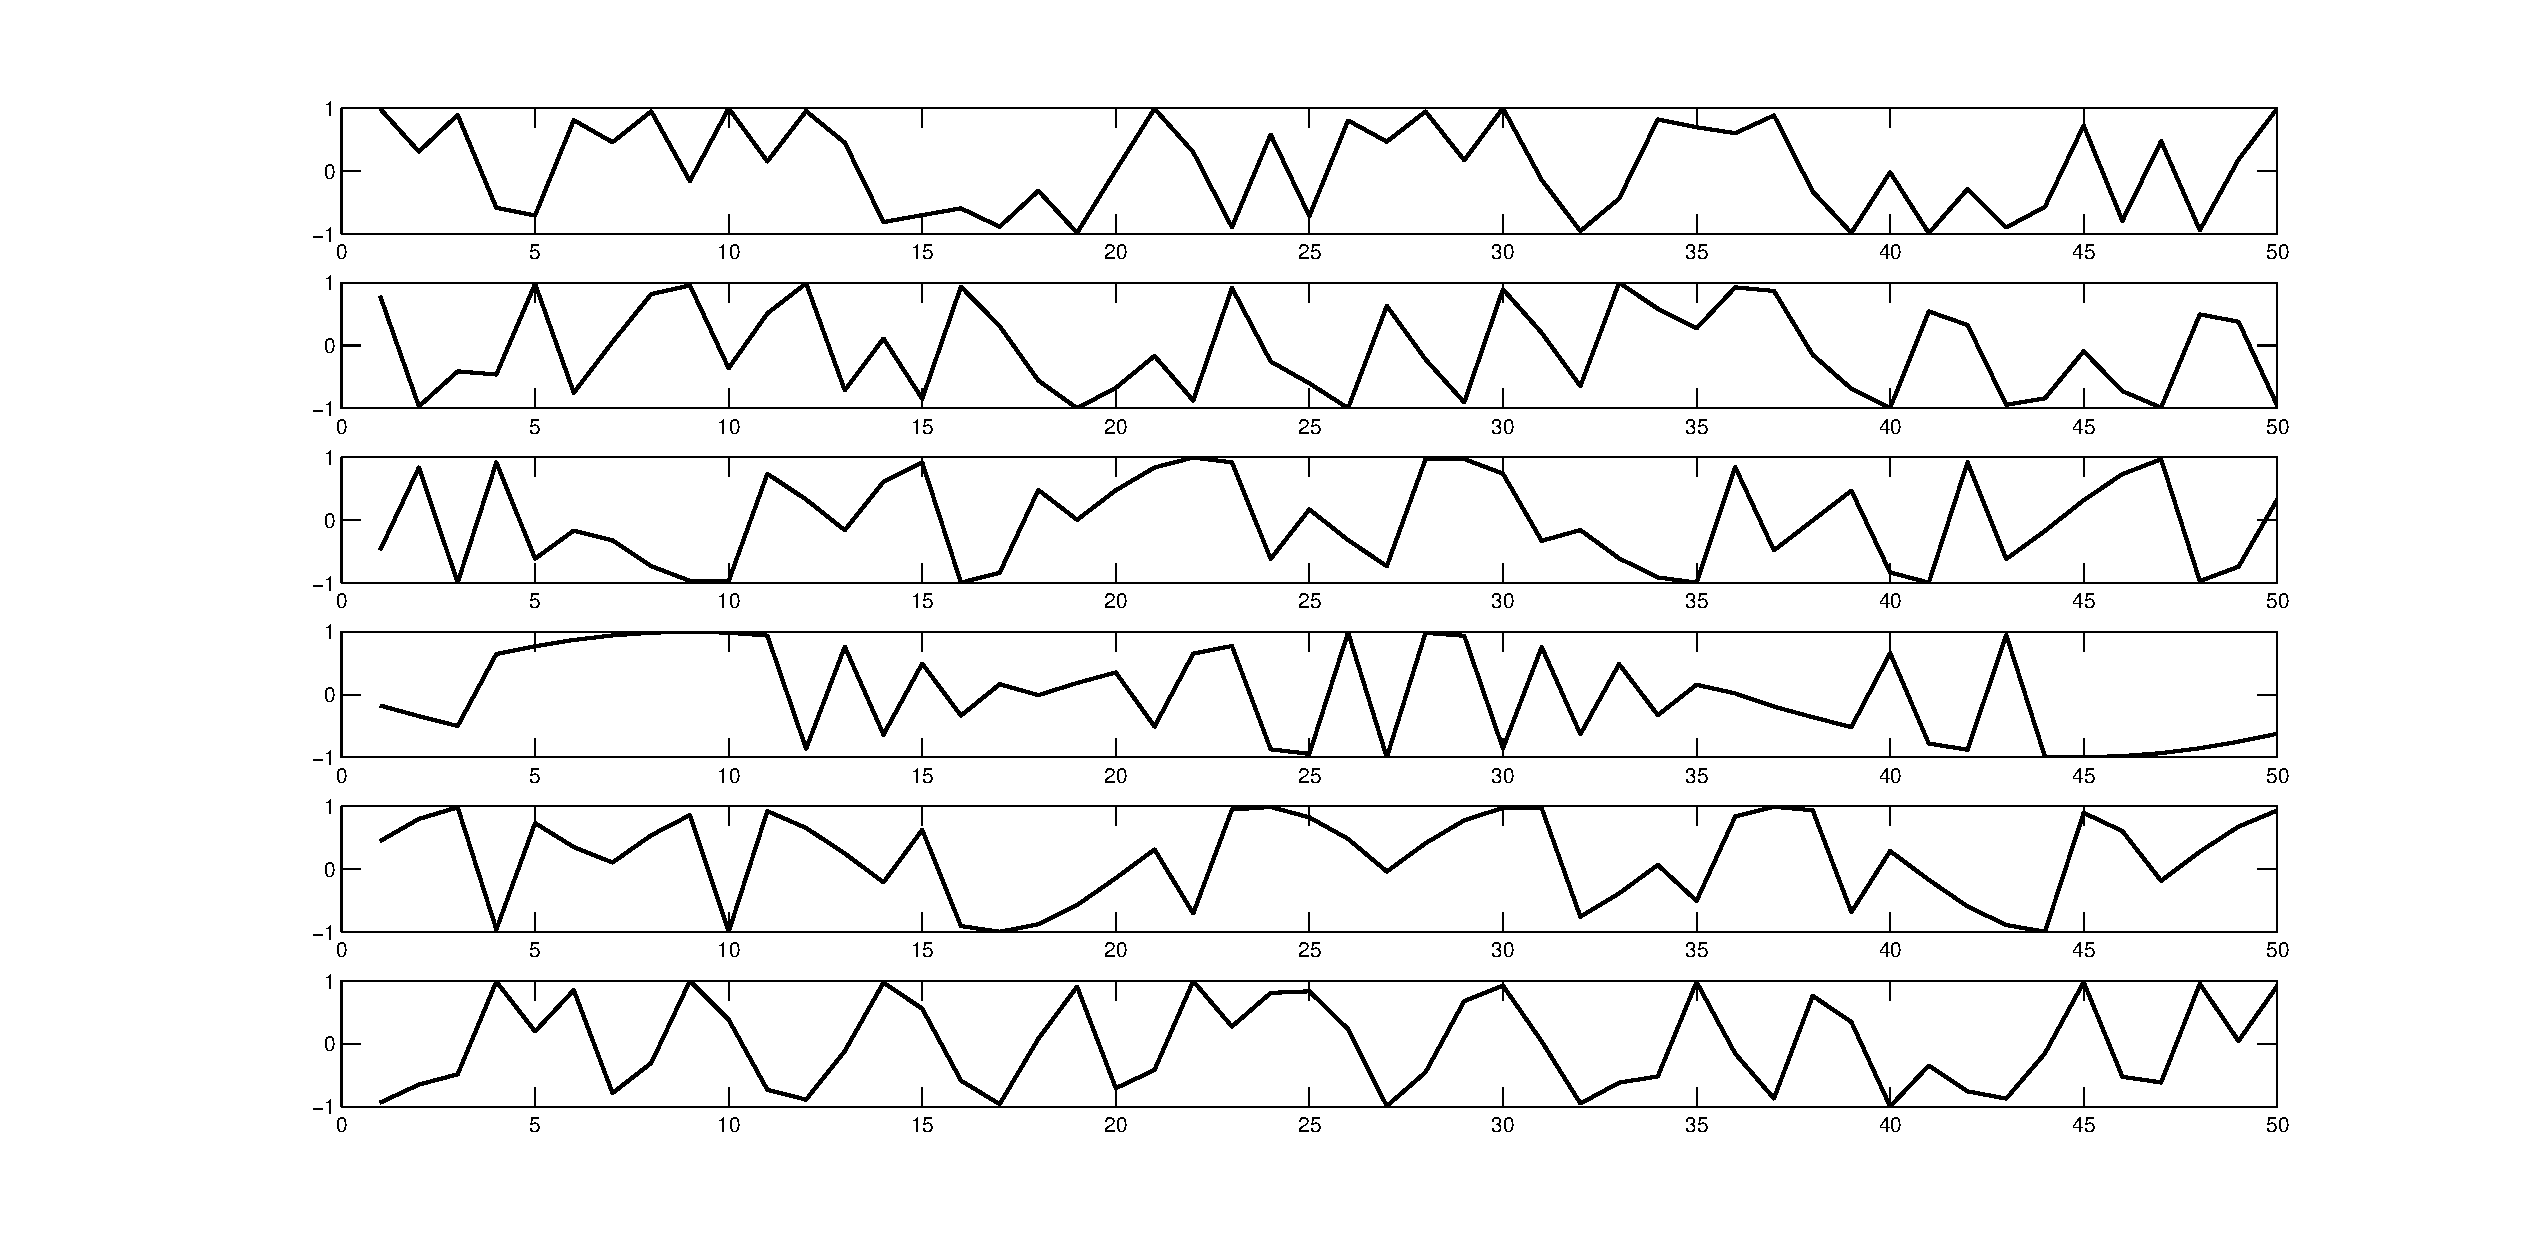
\includegraphics[width=0.75\textwidth]{Diagrams/Hidden-noisefree}
\ec

%Noisy BPSK sources:
%\bc
%\includegraphics[width=0.5\textwidth]{Diagrams/Hidden-noisy}
%\ec
}

\if0
\frame{
\frametitle{Observations}

Noise-free observation:
\bc
\includegraphics[width=0.5\textwidth]{Diagrams/Observed-noisefree}
\ec

Noisy observation:
\bc
\includegraphics[width=0.5\textwidth]{Diagrams/Observed-noisy}
\ec

}
\fi

\frame{
\frametitle{Example reconstructions: Noise-free case}
%Noise-free BPSK sources:
%\bc
%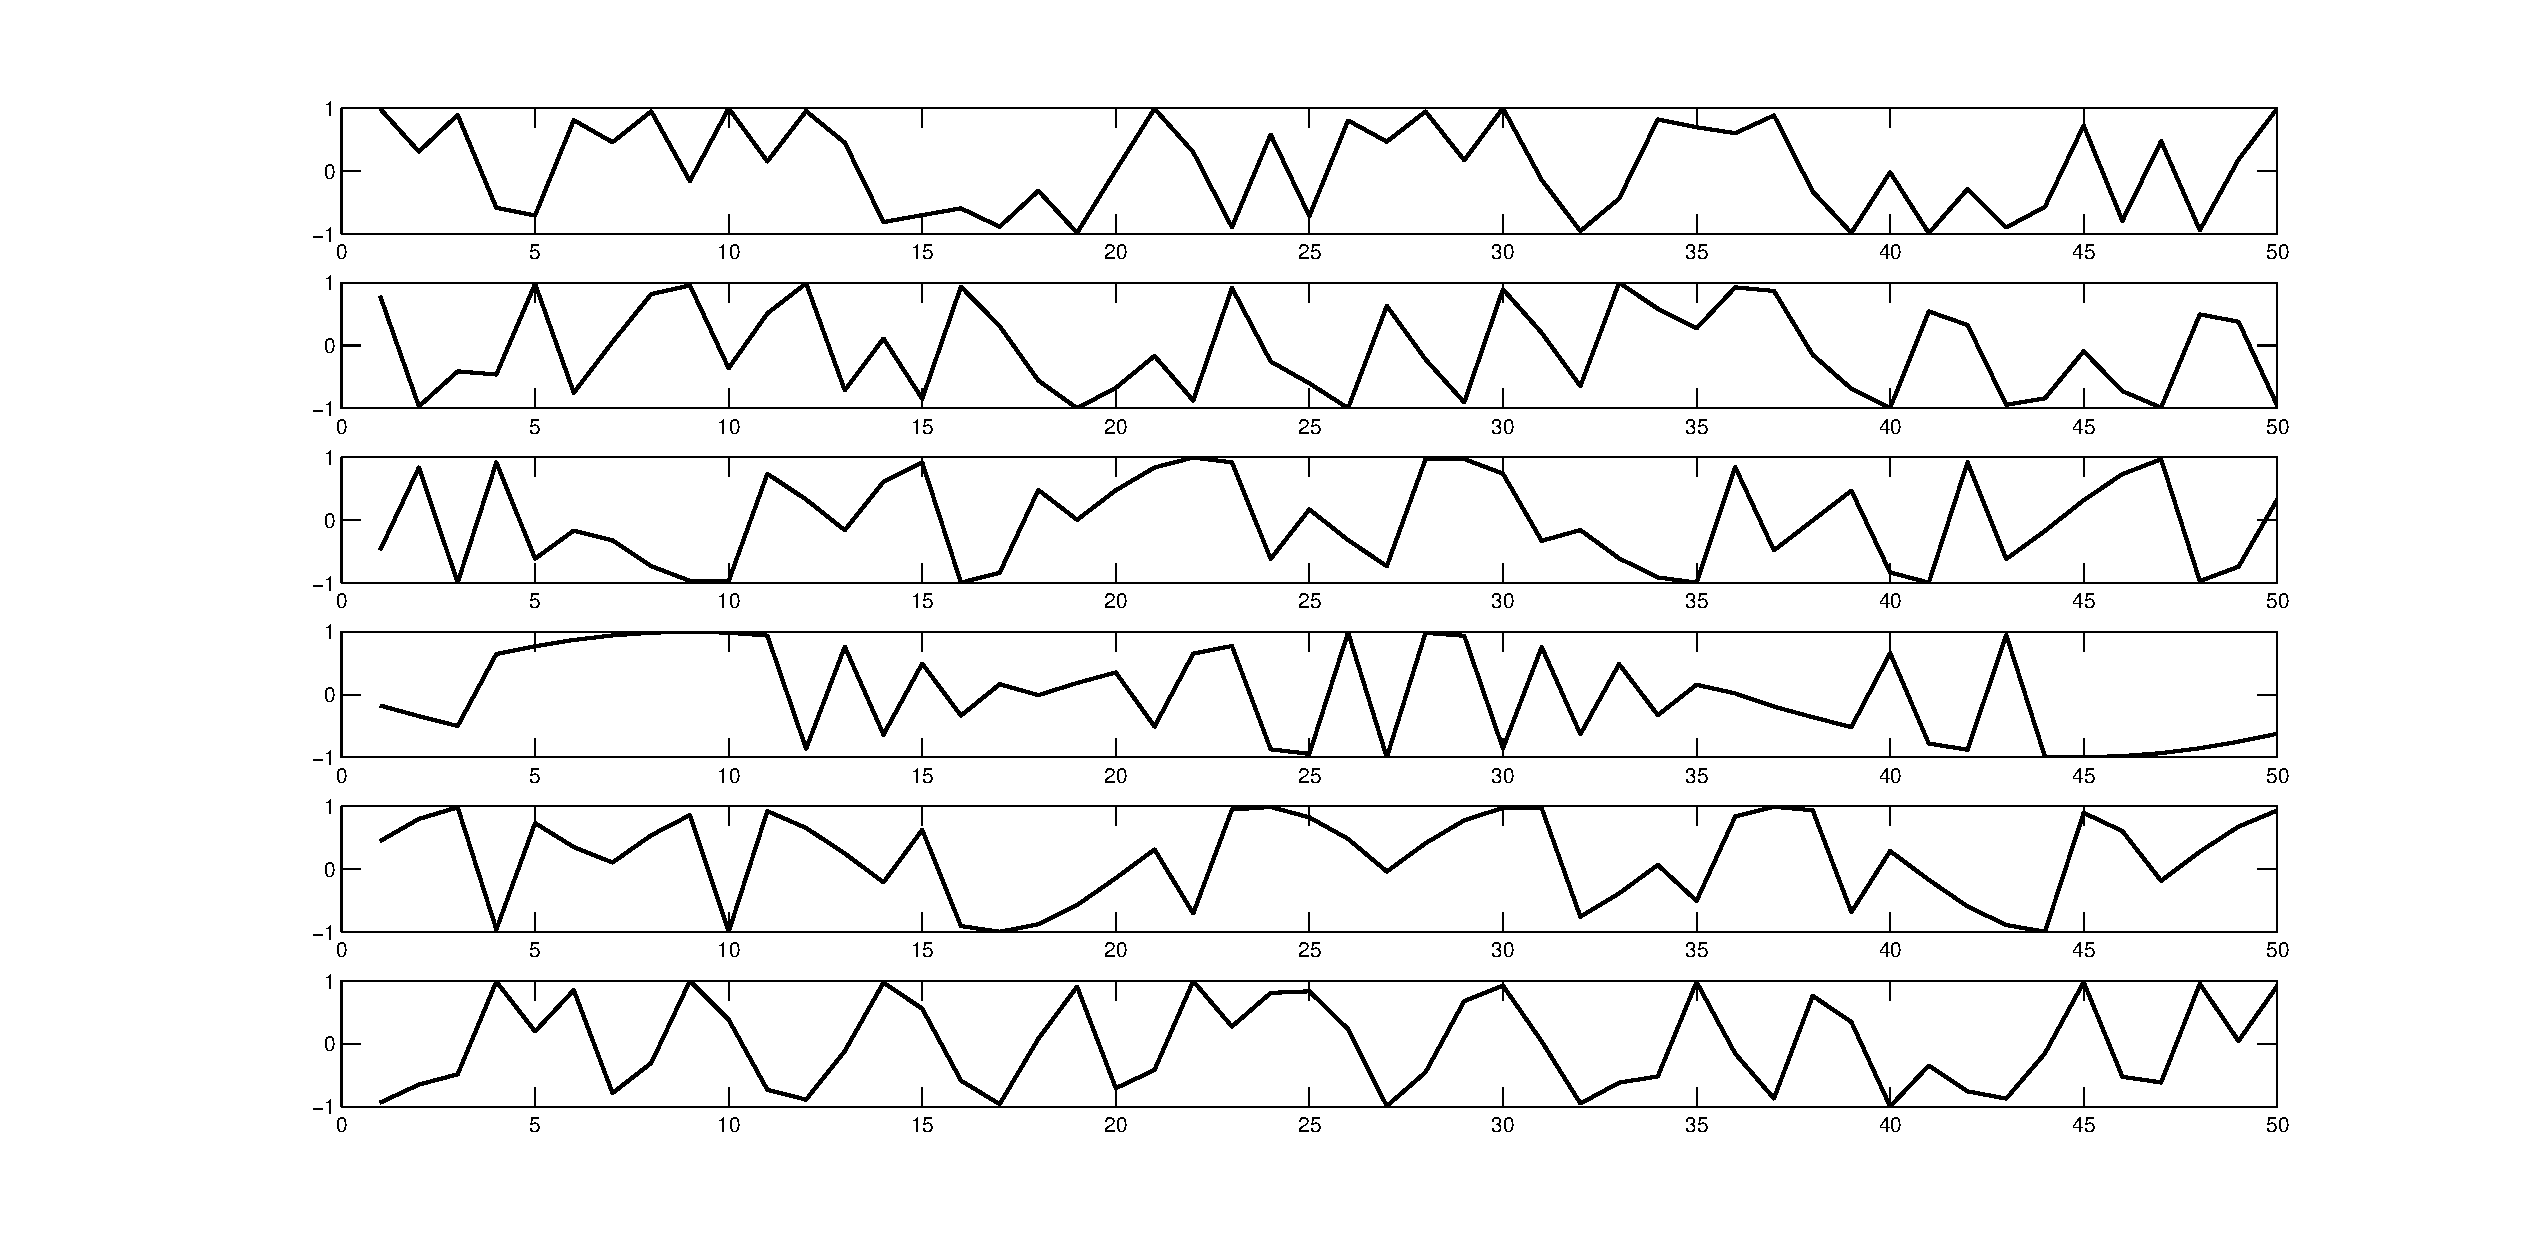
\includegraphics[width=0.75\textwidth]{Diagrams/Hidden-noisefree}
%\ec

Reconstruction:
\bc
\includegraphics[width=0.75\textwidth]{Diagrams/Reconstructed-noisefree}
\ec

}

\if0
\frame{
\frametitle{Example reconstructions: Noisy case}
Noisy-free BPSK sources:
\bc
\includegraphics[width=0.5\textwidth]{Diagrams/Hidden-noisy}
\ec

Reconstruction:
\bc
\includegraphics[width=0.5\textwidth]{Diagrams/Reconstructed-noisy}
\ec

}
\fi

\frame{
\frametitle{Noise: reconstruction of $A_1$}

\bc
\includegraphics[width=0.8\textwidth]{Diagrams/barchart-A1-noise}
\smallskip

\small
Reconstruction error of ``random'' matrix: $0.9\pm0.033$.\\
Error bars are based on $150$ runs.
\ec
}


\frame{
\frametitle{Coherence}
\begin{columns}[t]
\column{0.5\textwidth}

\includegraphics[width=\textwidth]{Diagrams/barchart-A1toA4-noisy}
\bc\small standard
\ec
\column{0.5\textwidth}

\includegraphics[width=\textwidth]{Diagrams/barchart-A1toA4-noisy_scaled}
\bc\small normalized
\ec
\end{columns}

}


\frame{
\frametitle{Recursive versions}
\bc
\includegraphics[width=0.7\textwidth]{Diagrams/barchart-recursive-noisy}
\ec
}


%\frame{
%\frametitle{
\if0
\vspace{-1cm}
\bi 
\item 9 different algorithms: 
	\bi
	\item<1-> HKICA (HKICA), and its recursive version (HKICA.R); 
	\item<1-> DICA  (DICA), and its recursive version (DICA.R); 
	\item<1-> A heuristic modification of  DICA  (MDICA), and its recursive version (MDICA.R);
	\item<1-> The default FastICA algorithm \citep{szabo12separation} (FICA);
	\item<1-> The recursive Fourier PCA \citep{vempala2014max}(FPCA);
	\item<1-> Random guessing (Random).
	\ei
\item 5 types of mixing matrices:
	\bi 
	\item<2-> $A = R$ is an orthonormal matrix;
	\item<2-> $A(A_1) = P$; 
	\item<2-> $A(A_2) = v_b\times\boldsymbol{1}' + 0.3\times P$;
	\item<2-> $A(A_3) = v_b\times\boldsymbol{1}' + 0.05\times P$;
	\item<2-> $A(A_4) = v_b\times\boldsymbol{1}' + 0.005\times P$  
	\item The vector $v_b$ and the matrix $P$ are both generated from standard normal distribution, and then normalized.
	\ei
\ei
}
\fi

\if0
\frame{ \frametitle{Setting}
\bi
\item 6-dimensional BPSK signals with different periods;
\item $x = As + c\eps$ for different noise ratio coefficients $c$;
\item $T = 20000$ observations;
\item Results are evaluated on a 150 repetitions. For each repetition, we try 3 times and report the best.
\ei
}

{\nologo
\frame{ \frametitle{Simulation resutls}
\begin{multicols}{3}
	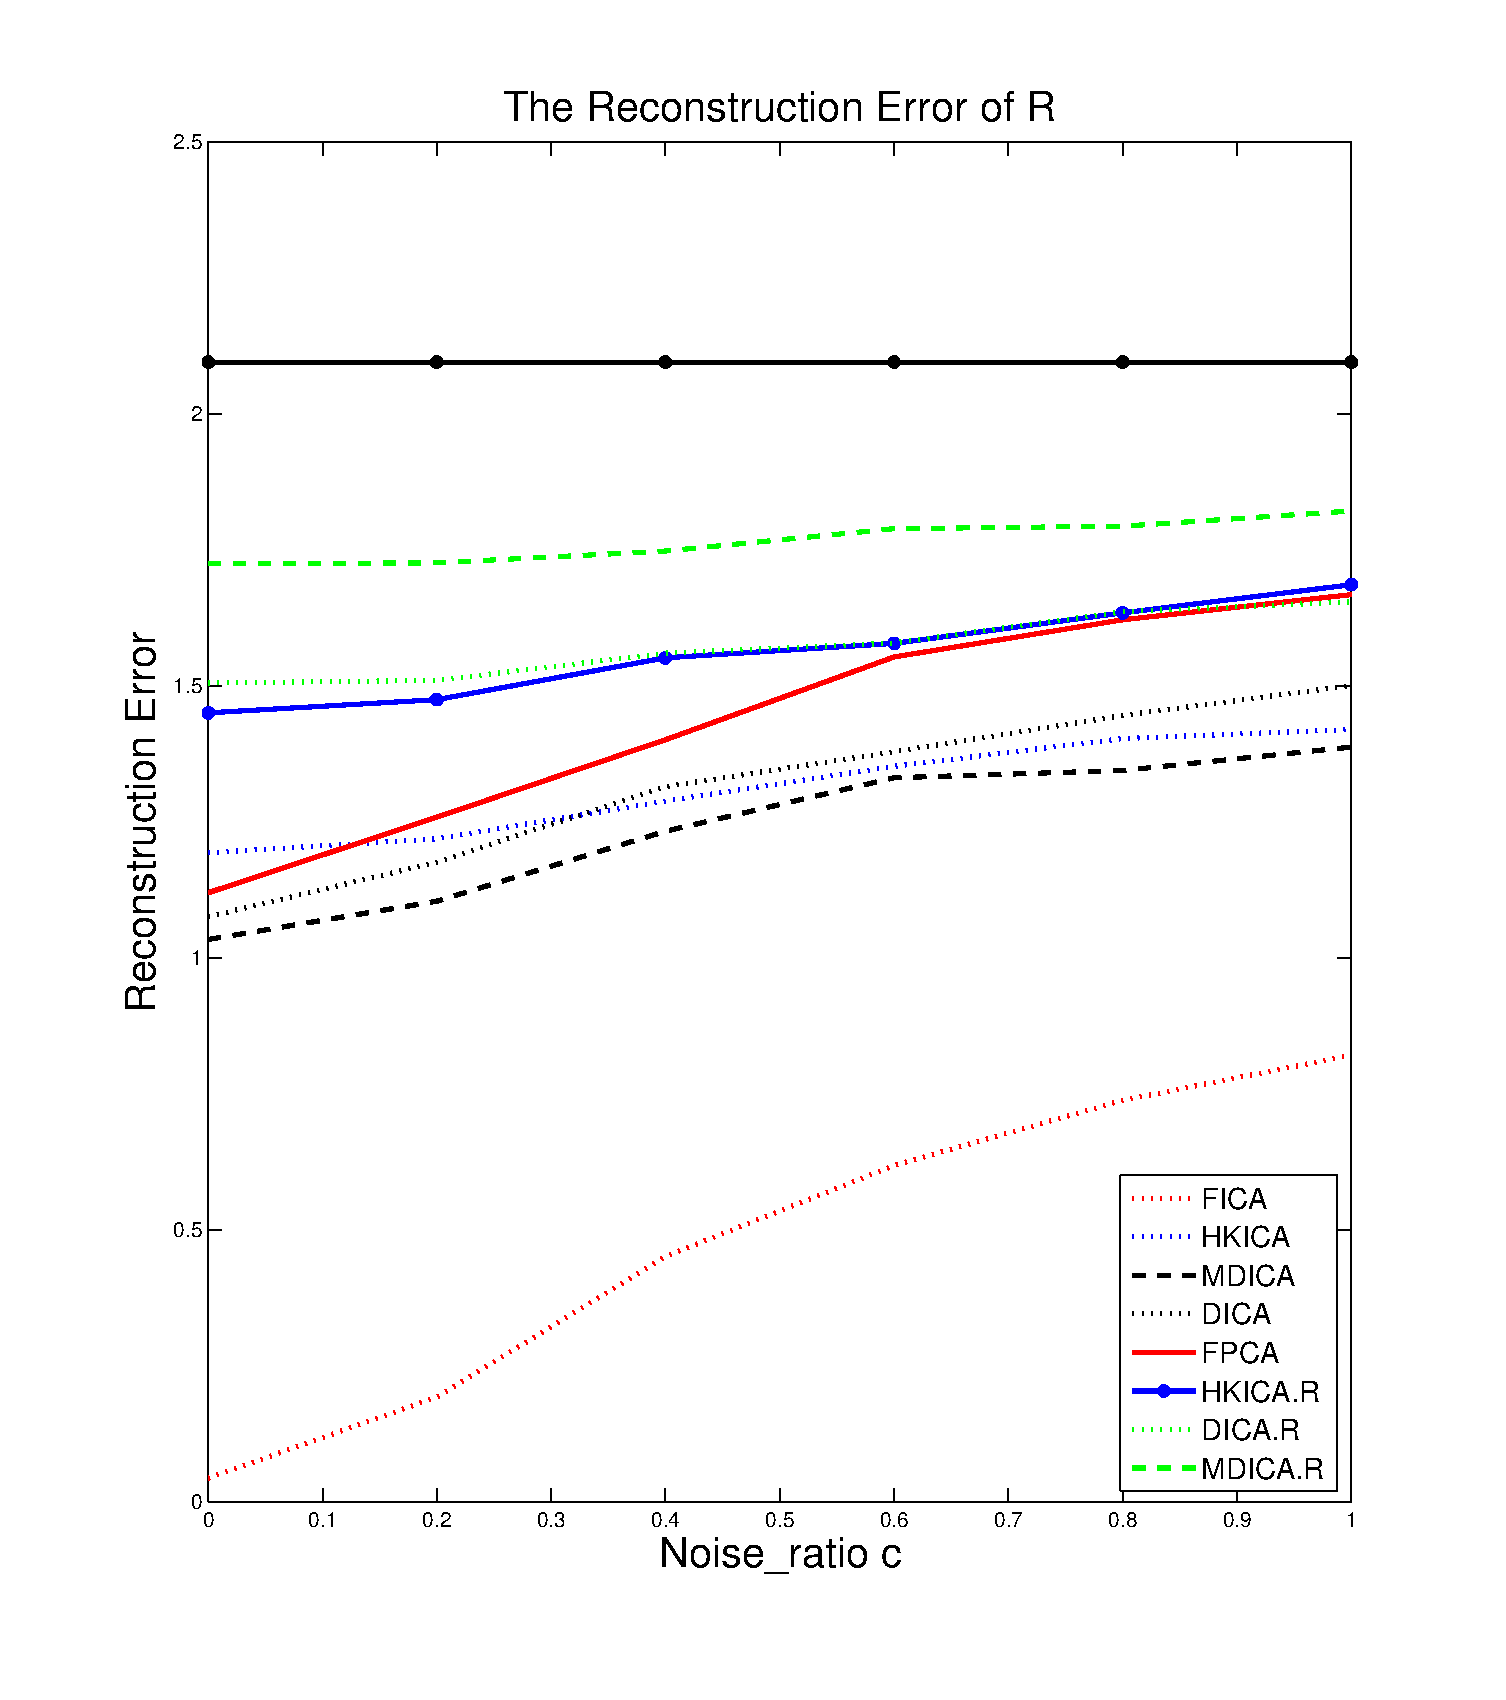
\includegraphics[height = 0.42\textheight]{errorR}\\
	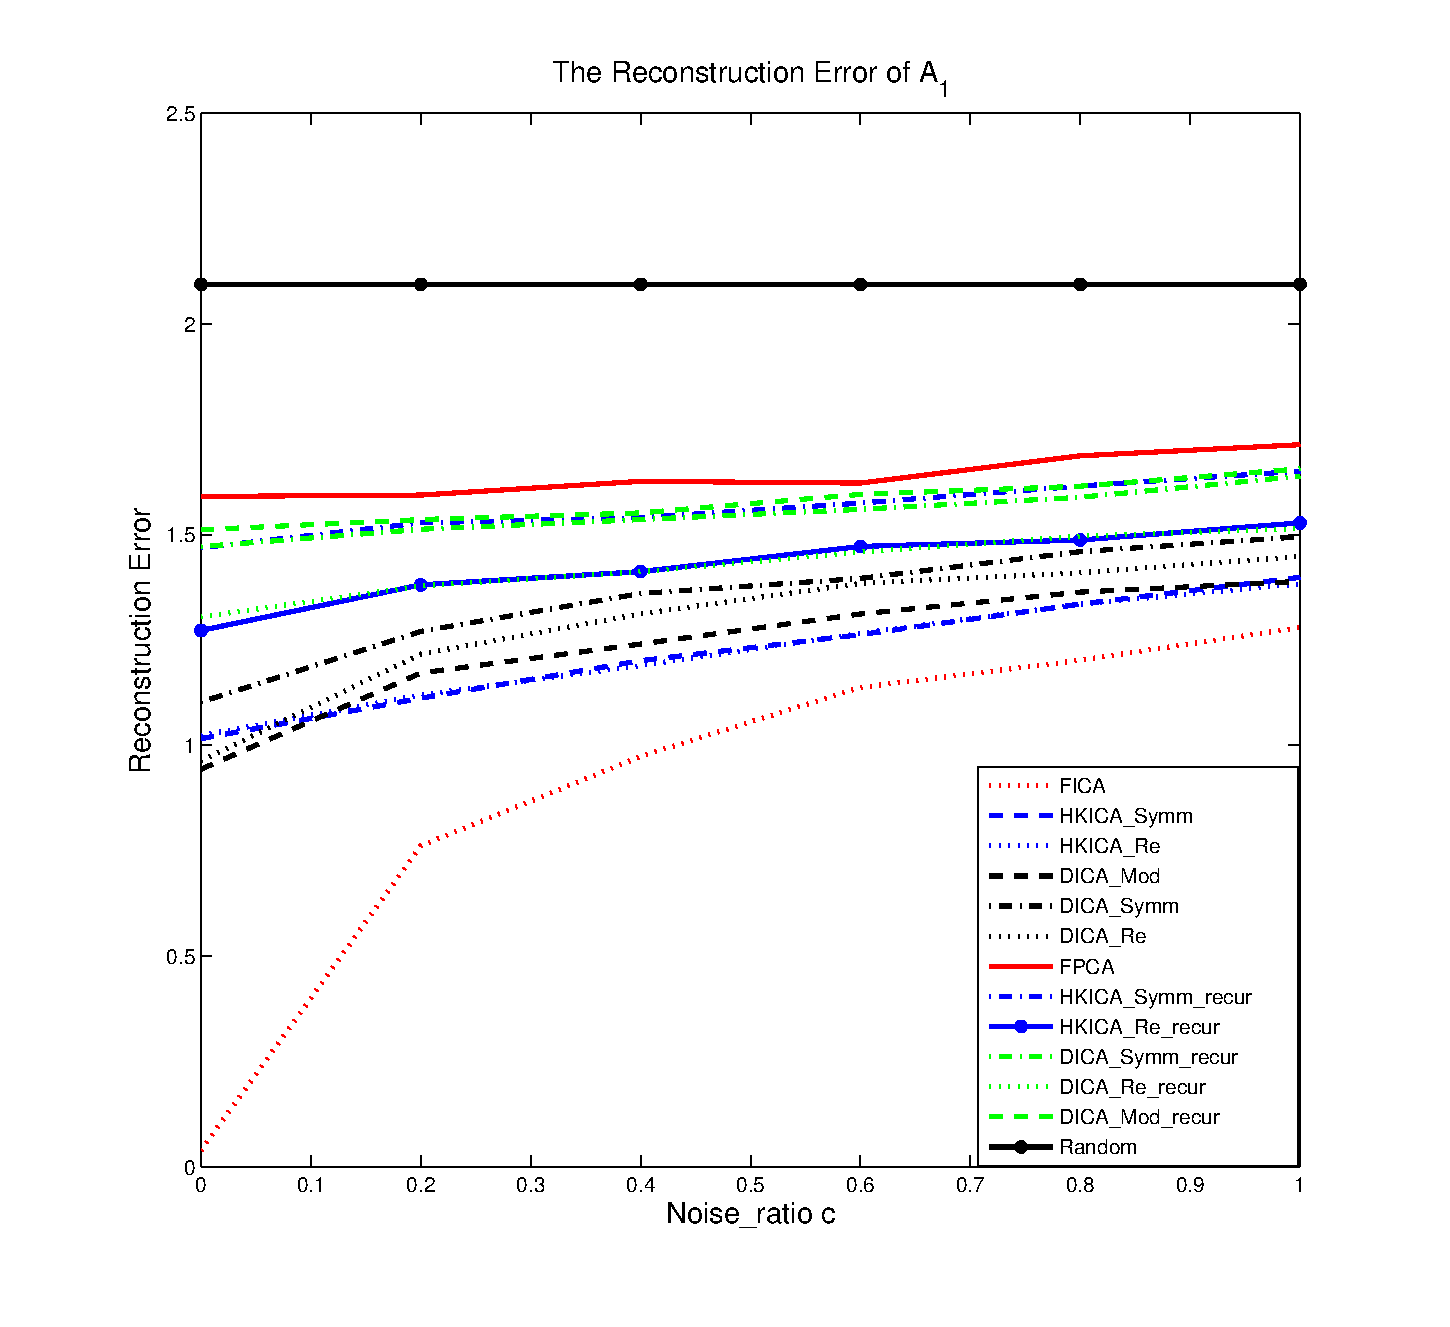
\includegraphics[height = 0.42\textheight]{error1}
	\newpage
	\topskip0pt
	\vspace*{\fill}
	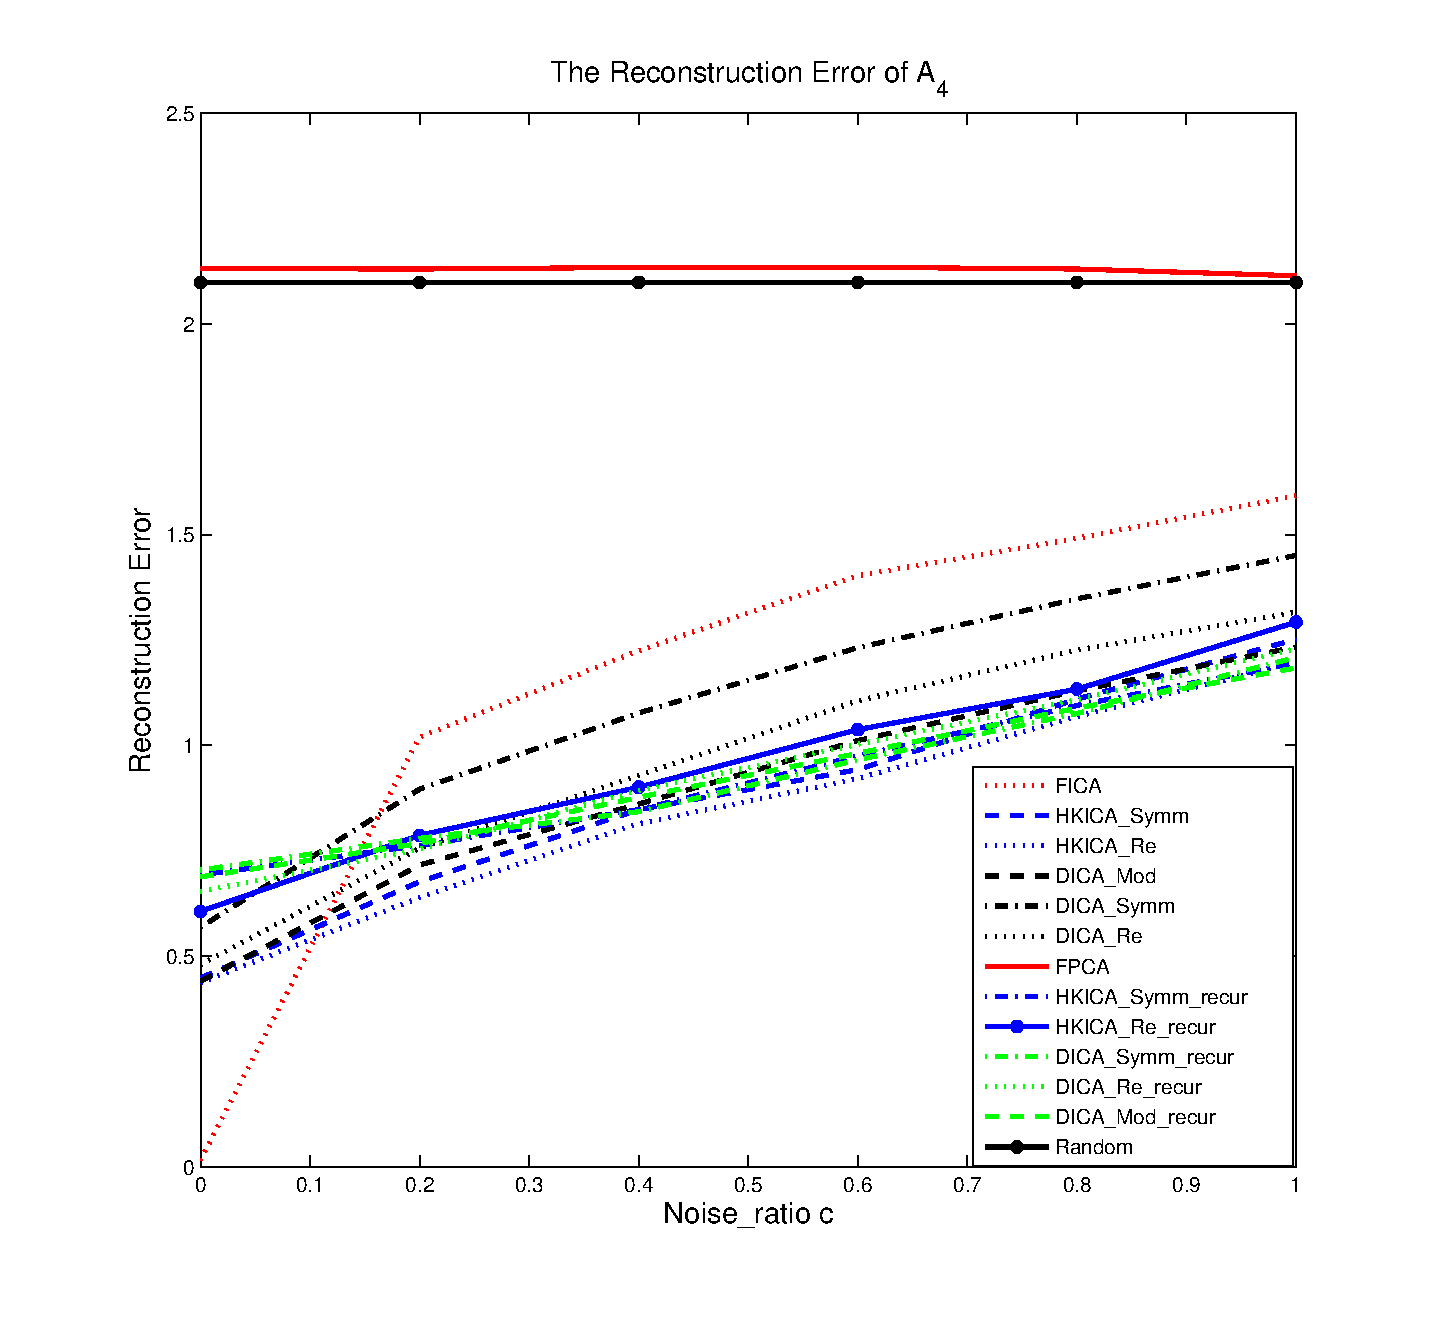
\includegraphics[height = 0.42\textheight]{error2}
	\vspace*{\fill}
	\newpage
	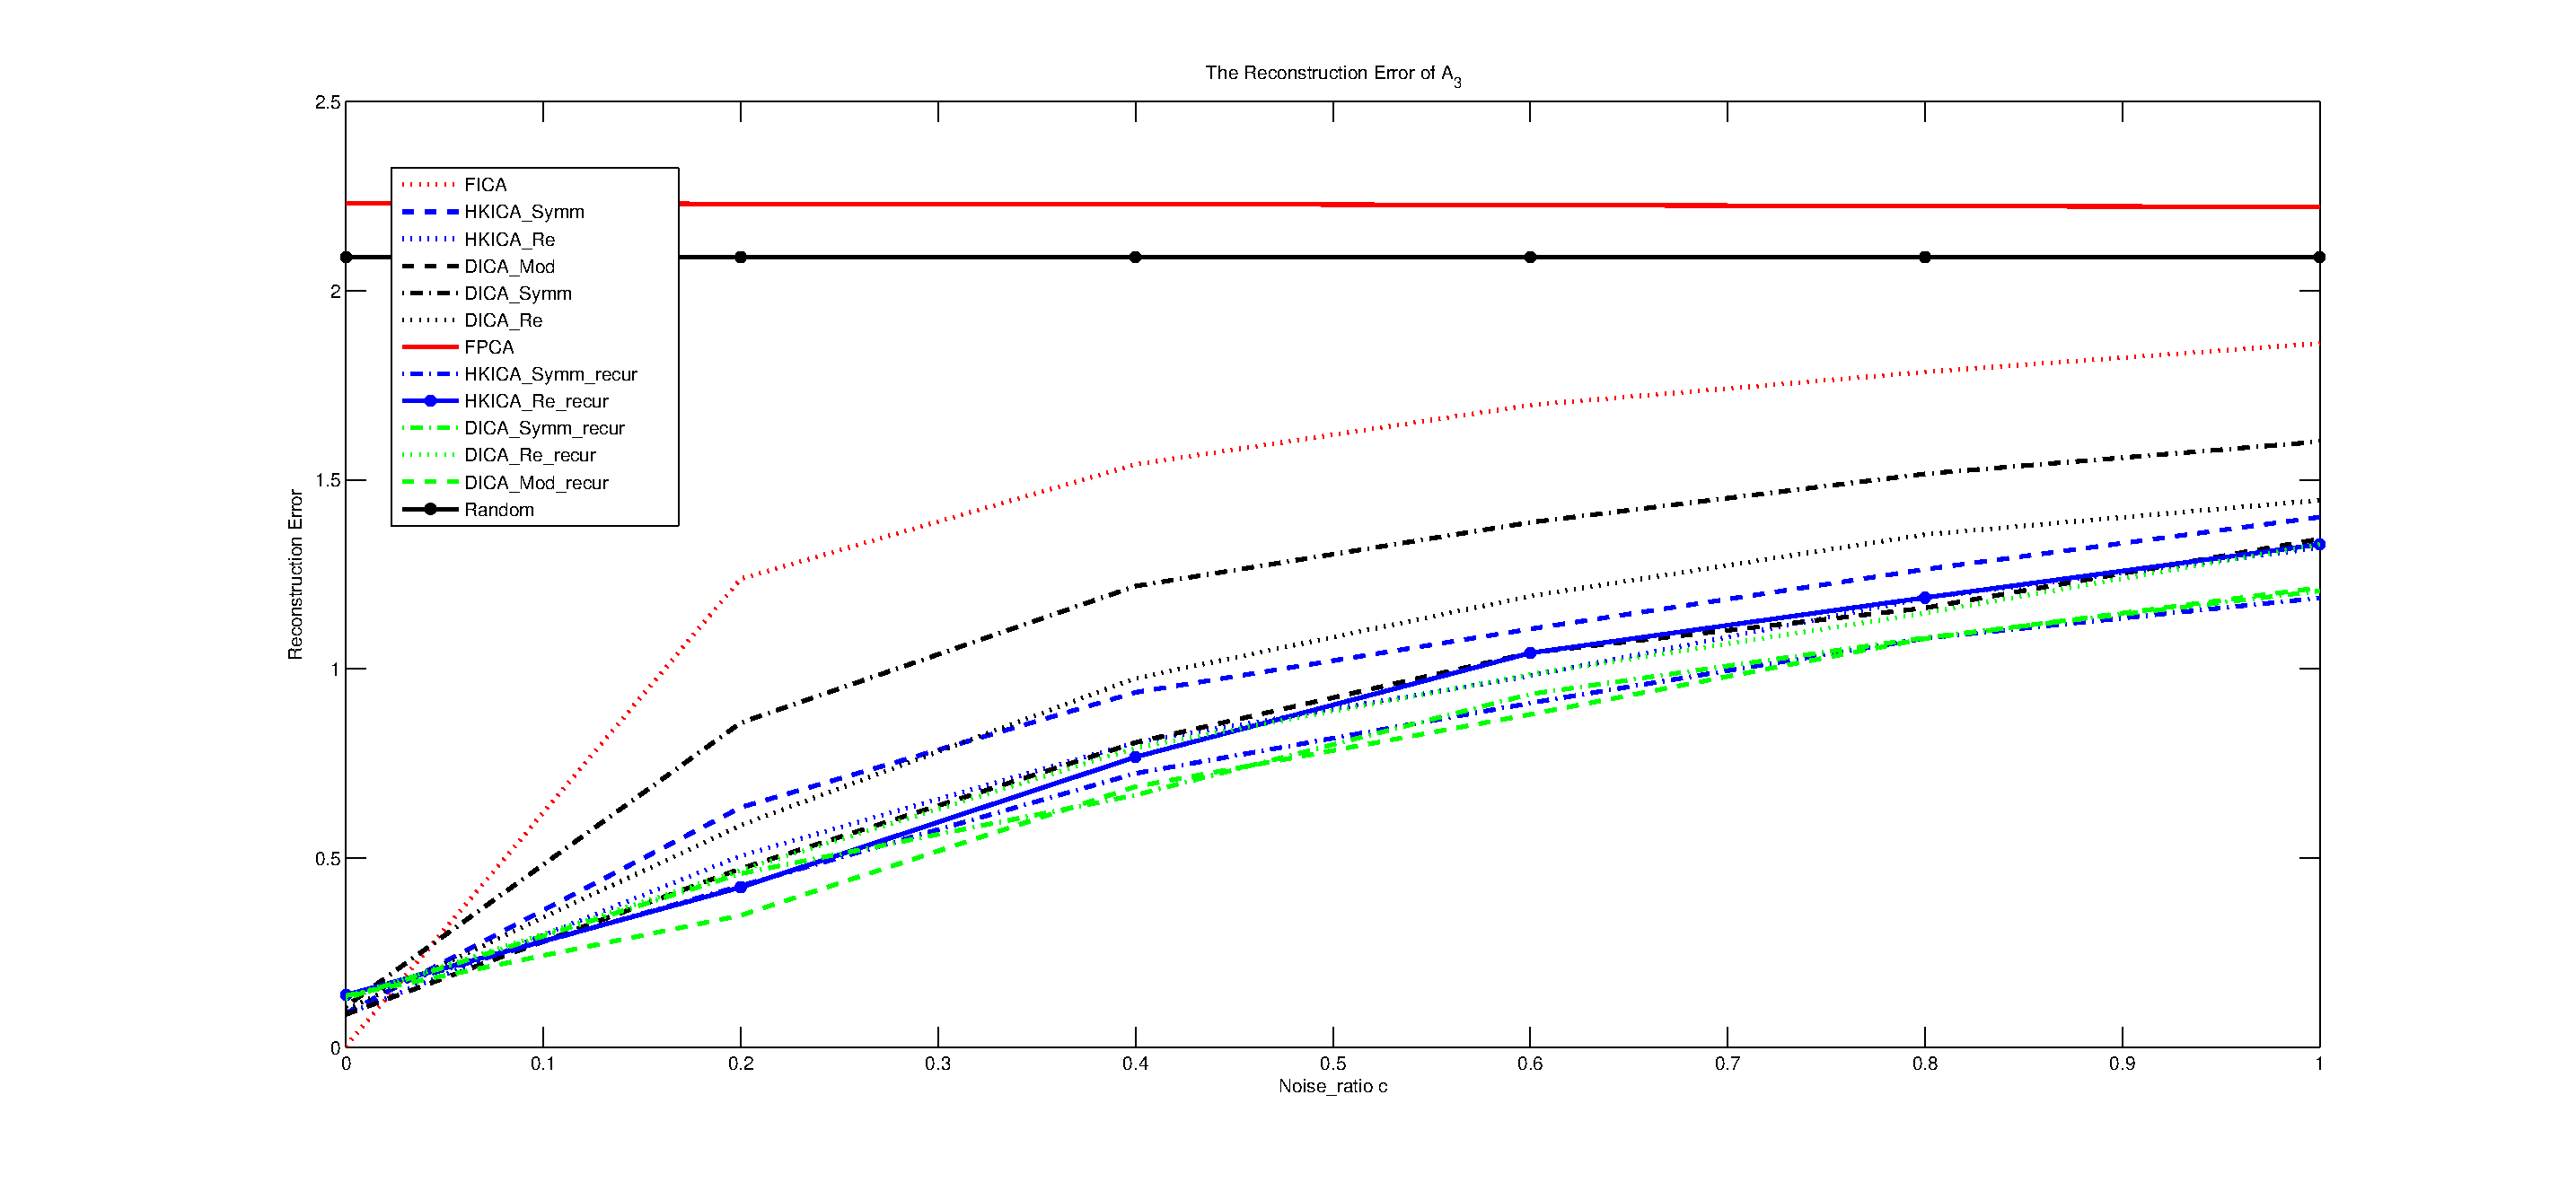
\includegraphics[height = 0.42\textheight]{error3}\\
	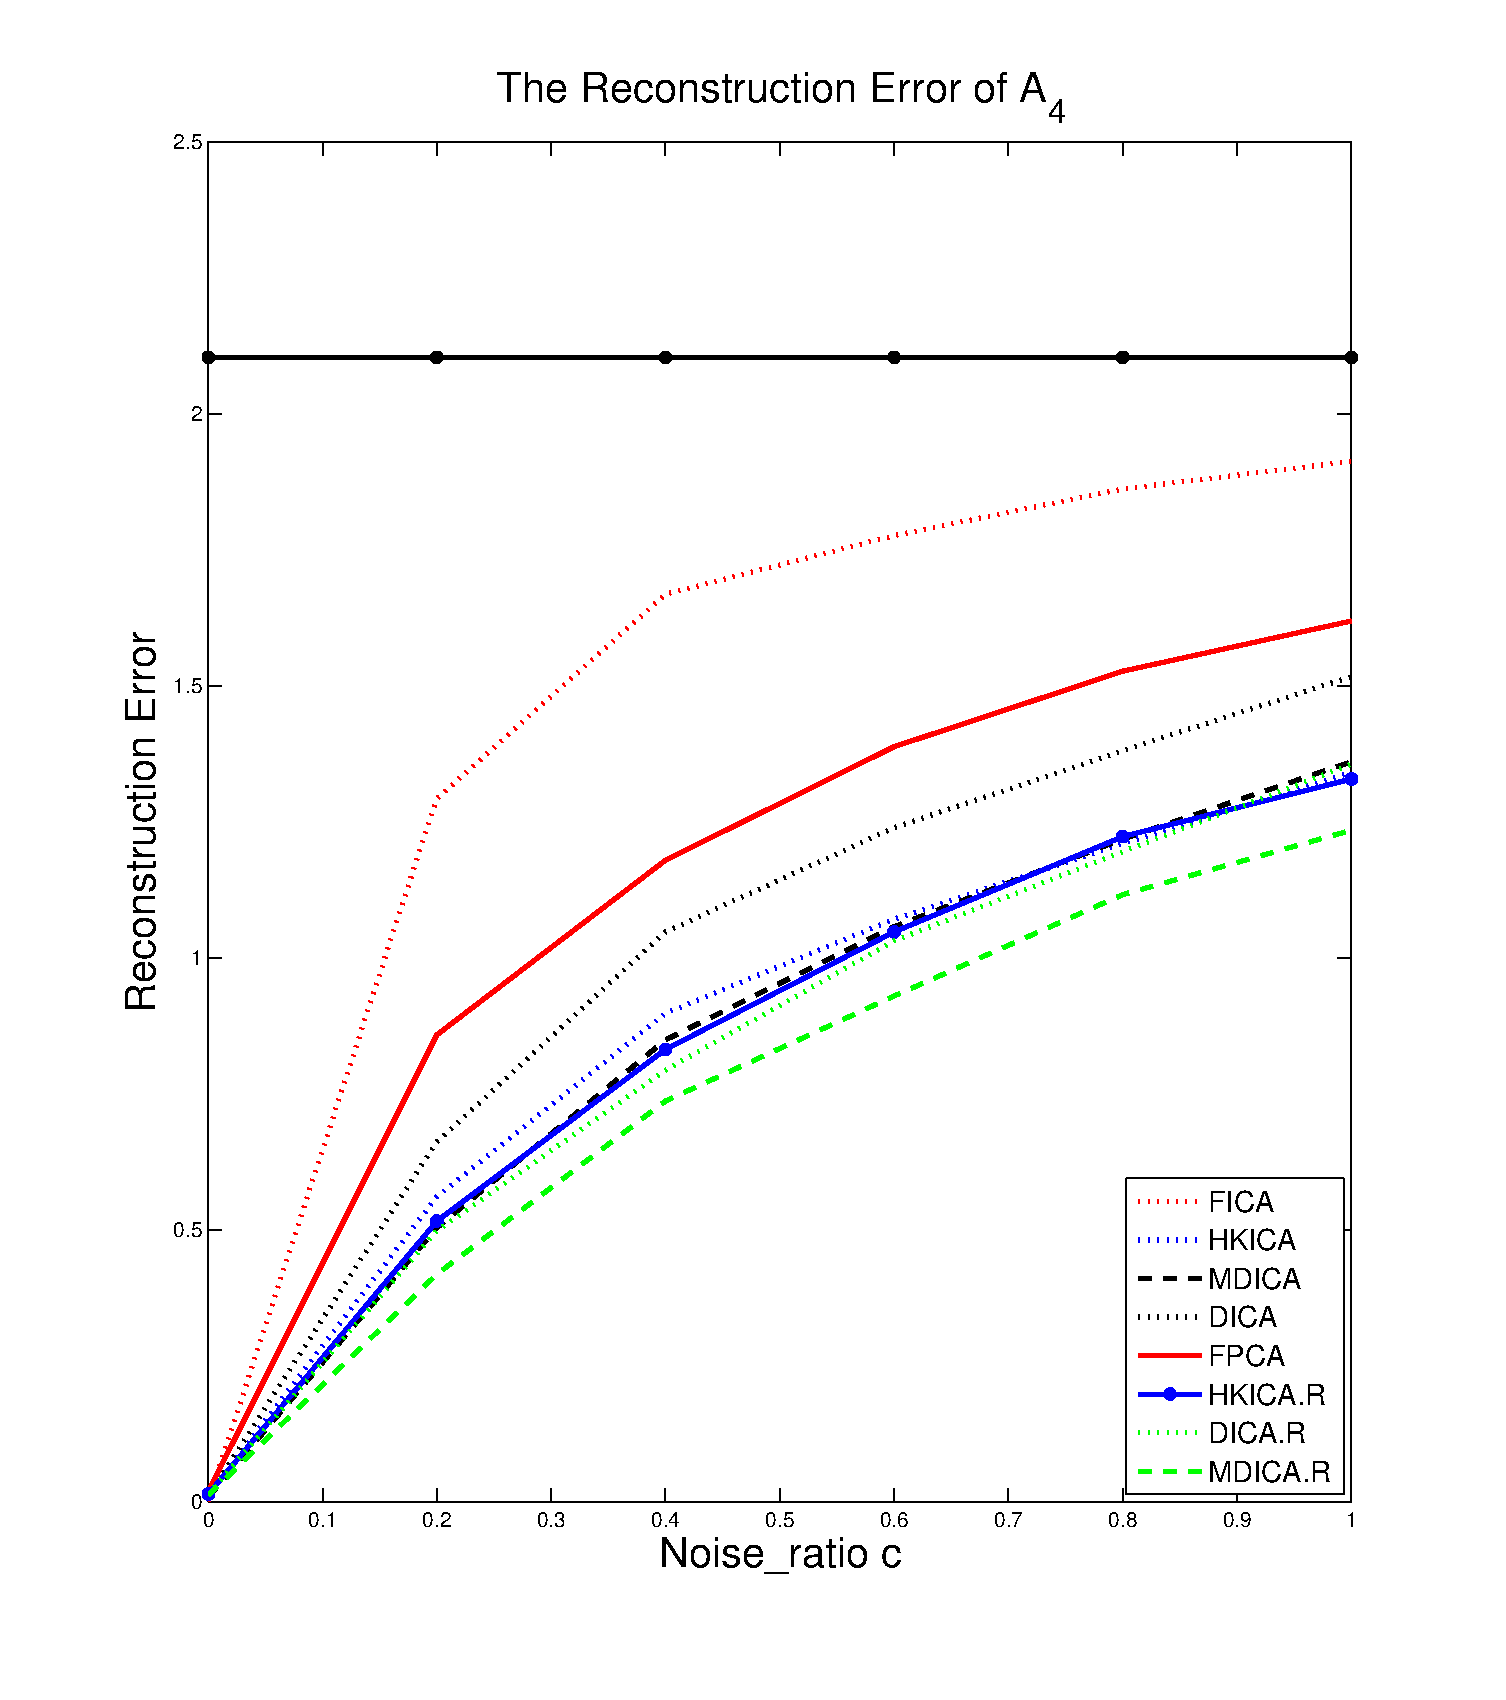
\includegraphics[height = 0.42\textheight]{error4}
\end{multicols}
}
}
\fi

\frame{
\centering
\color{blue}{
\Huge Big Picture
}}
\section{Big Picture}

%\begin{frame}{Outline}
%\tableofcontents[currentsection]
%\end{frame}

\frame{\frametitle{Statistical Unsupervised Learning (Generative)}
\begin{center}
\includegraphics[width=\textwidth]{StatLearning}
\end{center}
}

\frame{\frametitle{Agnostic Statistical Unsupervised Learning (New, \footnotesize{unexplored})}
\begin{center}
\includegraphics[width=\textwidth]{StatAgnosticLearning}
\end{center}
}

\frame{\frametitle{Agnostic \sout{Statistical} Unsupervised Learning (New: \footnotesize{This work})}
\begin{center}
\includegraphics[width=\textwidth]{AgnosticLearning}
\end{center}
}


%\section{Conclusions}
%
%\begin{frame}{Outline}
%\tableofcontents[currentsection]
%\end{frame}
%
\frame{\frametitle{ICA Conclusions}
\bi
\item Independent Component Analysis without generative models! 
\item New method: DICA. Universal, strong guarantees. Reproduces and strengthens previous results.
\item In practice, moment-methods are indeed more robust to noise.
\item Deterministic analysis: Cleaner, more general, should do it more often! Limits? Lower bounds?
\item Questions:
\bi
\item What is the effect of coherence? How to normalize the error measure properly?
\item HKICA is great! Why? MDICA is also good. Why?
\item ``Recursive versions'': No significant advantage was found (limited study?).
\ei
\ei
\medskip
\uncover<+->{Code: \url{https://github.com/Armstring/Deterministic-ICA}}
}


\frame{
\centering
\color{blue}{
\Huge Example 2: Follow the leader and fast rates in online linear optimization
}}


\begin{frame}{Follow the leader and fast rates in online linear optimization}
\linespread{1.9}
\bi
\item Follow the leader is the most intuitive online learning algorithm
\item Its performance can be extremely good or bad, depending on the circumstances
\item \alert{Goal:} Identify the conditions when it works well
\ei
\end{frame}



\begin{frame}{Online linear optimization}
Problem setup: compact, convex constraint set $\cW \subset \R^d$, set of loss vectors $\cF \subset \R^d$.

In every round $t=1,2,\ldots$:
\begin{itemize}
\item Learner predicts $w_t\in \cW$. 
\item Environment picks a loss function $f_t \in \cF$. 
\item Learner suffers loss $\ip{w_t,f_t}$ and observes $f_t$.
\end{itemize}
\pause
Goal: minimize regret
\vspace{-0.2cm}
\[
R_n = \sum_{t=1}^n \ip{w_t,f_t} - \min_{w\in \cW}\sum_{t=1}^n \ip{f_t,w}\,.
\]
%\smallskip
\pause
\vspace{-0.2cm}
\begin{block}{Follow the leader (FTL)}
\vspace{-0.1cm}
\[
w_t = \argmin_{w\in \cW} \sum_{i=1}^{t-1} \ip{f_i,w}
\]
\vspace{-0.3cm}
\end{block}
\end{frame}


\begin{frame}{FTL: ups and downs}
\begin{itemize}
\item Minimax regret in online convex optimization: $O(\sqrt{n})$.
\item Fast rates on some easy data, e.g., exp-concave loss functions: $O(\log(n))$ regret.
\pause
\item FTL with two experts can be
\end{itemize}
\bigskip
%\bigskip
\hspace{0.2cm}
\begin{minipage}{0.45\textwidth}
\begin{center}
\small
arbitrarily bad \\
$\left[\begin{array}{cccccc} 0.5 & 0 & 1 & 0 & 1 & \ldots \\ 0 & 1 & 0 & 1 & 0 & \ldots\end{array}\right]$ 
\includegraphics[width=0.9\textwidth]{figures/FTL-hard}
\end{center}
\end{minipage}
\begin{minipage}{0.1\textwidth}\end{minipage}
\pause
\begin{minipage}{0.45\textwidth}
\begin{center}
\small
extremly good \\
$\left[\begin{array}{cccccc} 0 & 0 & 1 & 0 & 1 & \ldots \\ 1 & 1 & 0 & 1 & 0 & \ldots\end{array}\right]$ 
\includegraphics[width=0.9\textwidth]{figures/FTL-easy} \\
\end{center}
\end{minipage}
\scalebox{0.5}{\tiny Courtesy of Gergely Neu}
\vspace{-5cm}
\pause
\begin{center}
\begin{minipage}{0.6\textwidth}
\begin{alertblock}{}{ \bigskip \centering \Huge When is FTL good? \bigskip}\end{alertblock}
\end{minipage}
\end{center}
\vspace{3cm}

\end{frame}


\begin{frame}{Fast rates in online convex optimization}
\begin{itemize}
\item Curved loss functions: strongly convex, exp-concave {\tiny \citep{MF92,hazan2007logarithmic,bartlett2007adaptive,kakade2009mind,orabona2012beyond,vanerven2015fast}}
\item Small loss of the optimal predictor {\tiny \citep{FrSc97}}
\item Small variations of losses {\tiny  \citep{RakhlinS13}}
\end{itemize}

\bigskip
\pause
\begin{alertblock}{}\centering{This talk: curvature of the constraint set helps!}
\end{alertblock}
\begin{itemize}
\item Already used in convex optimization 
\begin{itemize}
\item optimization over strongly convex constraint sets {\tiny \citep{LePo66,garber2014faster}}
\end{itemize}
\end{itemize}
\pause
\begin{block}{}\centering {Other easy problems for FTL}\end{block}
\end{frame}


\begin{frame}{FTL and the Support Function}
Support function of $\cW$:
\qquad $
\Phi(\Theta) = \max_{w\in\cW} \ip{w, \Theta}
$
\medskip

Average negative loss:
\qquad \quad$\displaystyle
\Theta_t = -\frac1t \sum_{i=1}^t f_i
$

\medskip
\pause
\begin{block}{FTL}
If $\Phi$ is differentiable at $\Theta_{t-1}$, $w_t=\nabla \Phi(\Theta_{t-1})$.
\end{block}

\medskip
\pause
\begin{alertblock}{Regret of FTL: }
\[
R_n = \sum_{t=1}^n t\,\ip{ w_{t+1}-w_t,\Theta_t} = \sum_{t=1}^{n} t\,D_{\Phi}(\Theta_t,\Theta_{t-1})
\]
{\tiny Bregman divergence: $D_{\Phi}(\theta', \theta) = \Phi(\theta') - \Phi(\theta) - \ip{ \nabla\Phi(\theta), \theta' - \theta}$}
\end{alertblock}

\begin{itemize}
\item[]
\begin{itemize}
\item Shows implicit connection with curvature...
\end{itemize}
\end{itemize}
\end{frame}


\begin{frame}{Curvature}
\footnotesize
\begin{itemize}
\item $\cW$ is $C^2$: the boundary $\bd(\cW)$ is a twice continuously differentiable submanifold of $\R^d$.
\item Gauss map: $u_{\cW} : \bd(\cW) \to \bS^{d-1}$  {\tiny(unit sphere)}
\begin{itemize}
\item continuously differentiable normal unit vector field
\end{itemize}
\item Principal curvatures: eigenvalues of  $\nabla u_{\cW}(p)$  
\begin{itemize}
\item eigenvalues of $\nabla^2 f(0)$ in the transformed coordinate system
\bigskip
\begin{center}
\hspace{-1cm}\includegraphics[width=0.55\textwidth]{figures/stronglyconvexset}
\end{center}
\smallskip
\item Example: principal curvatures of a sphere with radius $r$ are $1/r$.
\end{itemize}
\end{itemize}
\end{frame}

\begin{frame}{Examples}
The smallest principal curvature of some common convex bodies are as follows:
\begin{itemize}[<+->]\setlength{\itemsep}{10pt}
\item The smallest principal curvature $\lambda_0$ of the Euclidean ball $\cW = \set{w}{\|w\|_2\le r}$ of radius $r$ 
satisfies $\lambda_0=\frac{1}{r}$.
\item Let $Q$ be a positive definite matrix.
If $\cW = \set{w}{w^\top Q w\le 1 }$ then $\lambda_0=\lambda_{\min}/\sqrt{\lambda_{\max}}$, 
where $\lambda_{\min}$ and $\lambda_{\max}$ are the minimal, respectively, maximal eigenvalues of $Q$.
\item
In general, let $\phi:\R^d \to \R$ be a $C^2$ convex function.
Then, for $\cW = \set{w}{\phi(w)\le 1}$, 
$\lambda_0=\min_{w\in\bd(\cW)}\min_{v\,:\,\|v\|_2=1, v\perp \phi'(w) }\frac{v^{\top}\nabla^2\phi(w) v}{\|\phi'(w)\|_2}$~.
\end{itemize}
\end{frame}


\begin{frame}{Regret bound for FTL}
Assume
\begin{itemize}
\item $\cW\subset \R^d$ be a $C^2$ convex body (non-empty, compact) with $d \ge 2$;
\item the principal curvatures of the surface $\bd(\cW)$ are all at least $\lambda_0$ \\
\begin{itemize}
\item \small i.e., $\cW$ is $\lambda_0$-strongly convex;
\end{itemize}
\item $\Phi$ is differentiable at $(\Theta_t)_{t}$;
\item $M = \max_{f\in \cF} \norm{f}_2$
\item  $L_n:=\min_{1\le t \le n} \|\Theta_t\|_2 >0$. 
%\item $w_1\in \bd(\cW)$.
\end{itemize}
\begin{block}{}
Then
\[
R_n \le \frac{2M^2}{\lambda_0 L_n}(1+ \log(n))\,.
\]
\end{block}
\end{frame}

\if0
\begin{frame}{Strongly convex sets}
$\cW$ is $\lambda$-strongly convex with respect to the norm $\norm{\cdot}$ if, for  any $x,y\in \cW$ and $\gamma\in [0,1]$, the $\norm{\cdot}$-ball with origin $\gamma x + (1-\gamma) y$ and radius $\gamma(1-\gamma) \lambda \norm{x-y}^2/2 $ is included in $ \cW$. 

\bigskip

\pause

\begin{block}{Equivalence}
$\cW$ is $\lambda$-strongly convex with respect to $\norm{\cdot}_2$ if and only if the principal curvatures of the surface $\bd{\cW}$ are all at least $\lambda$.
\end{block}
\end{frame}

\begin{frame}{Strongly convex constraint sets}
Results in convex optimization:

\bigskip

\begin{itemize}
\item Exponential rates are attainable for strongly convex constraint sets if the norm of the gradients of the objective function admit a uniform lower bound. \citep{LePo66}
\bigskip
\item $O(1/n^2)$ optimization error bound (with problem-dependent constants) for the Frank-Wolfe algorithm for strongly convex and smooth objectives. \citep{garber2014faster}
\end{itemize}
\bigskip
\bigskip
\bigskip
\bigskip

\end{frame}
\fi

\begin{frame}{Regret lower bound}
Assume
\begin{itemize}
\item  $\lambda_0,L \in (0,1)$
\item $\seto{(-L,1), (-L,-1)} \subset \cF$ 
\item $\cW = \seto{(x,y):  \frac{x^2}{\lambda_0^2} + y^2 \le 1}$
\begin{itemize}
\item ellipsoid with minimal principal curvature $\lambda_0$.
\end{itemize}
\end{itemize}
\begin{block}{}
For any learning strategy, there exists a sequence of losses $f_1,f_2,\ldots \in \cF$ such that 
\[
R_n = \Omega\left(\frac{1}{L \lambda_0} \log(n)\right)
\]
and $\|\Theta_t\|_2 \ge L$ for all $t$.
\end{block}
\end{frame}

\begin{frame}{Intuition}
\begin{minipage}{0.55\textwidth}
\begin{itemize}
\item $\cW = \set{w}{\|w\|_2\le 1}$.
\item $f_t$ are i.i.d. with $\|f_t\|_\infty\le M$ and $\Exp{f_t} = \mu = (-1,0)$.
\item $w^* = (1,0)$, and thus $\inpro{w^*}{\mu} = -1$.
\item $E = \set{-\theta}{\|\theta - \mu\|_2 \le \epsilon}$, expect $-\mu_t \in E$ w.h.p. for $\epsilon=O(1/\sqrt{t})$.
\item Excess loss for $\mu_t$ is $| \tilde{B}D| \le |BD| \le  \epsilon^2 = O(1/t)$.
\item Overall regret: $O(\log(t))$
\end{itemize}
\end{minipage}\hspace{0.07\textwidth}
\begin{minipage}{0.35\textwidth}
\begin{center}
\includegraphics[width = \textwidth,
	trim={6.2cm 1cm 1.8cm 0},clip]
	{figures/ExcessError}
\end{center}
\end{minipage}
\end{frame}

%\begin{frame}{Proof of the lower bound}
%\begin{minipage}{0.55\textwidth}
%\begin{itemize}
%\item $\cW =  \seto{(x,y):  \frac{x^2}{\lambda_0^2} + y^2 \le 1}$.
%\item $f_t=(-L, 2 Y_t -1)$ where $Y_t \sim$ Bernoulli($p$).
%\item Beta prior on $p$ $\Rightarrow$ estimation error is $\Theta(1/\sqrt{t})$
%\item Compute the regret of the Bayes optimal strategy
%\end{itemize}
%\end{minipage}\hspace{0.07\textwidth}
%\begin{minipage}{0.35\textwidth}
%\begin{center}
%\includegraphics[width = \textwidth,
%	trim={6.2cm 1cm 1.8cm 0},clip]
%	{figures/ExcessError}
%\end{center}
%\end{minipage}
%\end{frame}



\begin{frame}{Proof sketch of the upper bound}
\begin{minipage}{0.57\textwidth}
Recall
\[
R_n = \sum_{t=1}^n t\,\ip{ w_{t+1}-w_t,\Theta_t}.
\]
\pause
%We will show:
\alert{Crucial step:}
\[
\ip{ w_{t+1}-w_t,\Theta_t} \le \frac{\|\Theta_t - \Theta_{t-1}\|_2^2}{2\lambda_0 \|\Theta_{t-1}\|_2}.
\]
\end{minipage}
\pause
\begin{minipage}{0.37\textwidth}
\begin{center}
\includegraphics[width=\textwidth, trim={4.8cm 1cm 3cm 0},clip]{figures/GaussmapPro}\end{center}
\end{minipage}
\vspace{-0.2cm}
\pause
Also, for $M = \sup_{f\in\cF} \|f\|_2$,
$\|\Theta_{t}-\Theta_{t-1}\|_2 \le \frac{2}{t} M.$
\pause

\bigskip
Then
\begin{align*}
R_n &= \sum_{t=1}^{n} t\ip{ w_{t+1}-w_t,\Theta_t} %\\ & 
\le \sum_{t=1}^{n} \frac{t}{2\lambda_0} \frac{\|\Theta_t - \Theta_{t-1}\|_2^2}{\|\Theta_{t-1}\|_2} \\
&\le \frac{2M^2}{\lambda_0}\sum_{t=1}^{n} \frac{1}{t\|\Theta_{t-1}\|_2} \le \frac{2M^2}{\lambda_0L_n} \sum_{t=1}^{n} \frac{1}{t}
\le \frac{2M^2}{\lambda_0L_n} (1+\log(n))\,.
\end{align*}
\end{frame}

\if0
\begin{frame}{Proof sketch of the upper bound}
\begin{minipage}{0.57\textwidth}
\small
\begin{align*}
w^{(i)} &= \argmax_{w\in\cW}\inpro{w}{\theta_i} \\
\ttheta_i &= \theta_i/\|\theta_i\|_2 \\
\text{$u_\gamma(s)$:} & \quad \text{projection of outer unit}\\[-0.5em] &\text{normal vector $u_{\cW}(w)$ to $P$}\\
\gamma(0)&=w^{(1)}, \qquad u_\gamma(0)=\ttheta_1 \\
\gamma(l)&=w^{(2)}, \qquad u_\gamma(l)=\htheta_2
\end{align*}
\end{minipage}\hspace{0.03\textwidth}
\begin{minipage}{0.37\textwidth}
\begin{center}
\includegraphics[width=\textwidth, trim={4.8cm 1cm 3cm 0},clip]{figures/GaussmapPro}\end{center}
\end{minipage}
\vspace{-0.2cm}
%\pause
\begin{itemize}
\item Curvature: $\|u'_\gamma(s)\|_2= \lambda(s) \ge \lambda_0$ and $\gamma'(s)=\frac{u'_\gamma(s)}{\|u'_\gamma(s)\|_2}$.
\item $\gamma$ can be selected so that $\ip{\gamma'(s),\ttheta_1} \le 0$. %$\Rightarrow$ $|u_\gamma'(s)\|_2 \inpro{\gamma'(s)}{\ttheta_1} \le \lambda_0 \inpro{\gamma'(s)}{\ttheta_1}$
\end{itemize}
%\vspace{-0.2cm}
%\pause
\begin{align*}
%\cos \inangle{\ttheta_1}{\ttheta_2} & \le 
\cos \inangle{\ttheta_1}{\htheta_2} &= 1 \! + \inpro{\htheta_2 - \ttheta_1}{\ttheta_1}  
= 1\!+ \!\int_{0}^{l} \inpro{u_\gamma'(s)}{\ttheta_1} \,\text{d}s  \\[0.3em]
&  \le 1 + \lambda_0 \int_0^l \ip{\gamma'(s),\ttheta_1}
 \le 1 - \lambda_0 \inpro{w^{(1)}  - w^{(2)}}{\ttheta_1}
\end{align*}
 

\end{frame}

\begin{frame}{Proof sketch of the upper bound}
From previous slide:
\[
\inpro{w^{(1)}  - w^{(2)}}{\ttheta_1} \le \frac{1-\cos \inangle{\ttheta_1}{\htheta_2}}{\lambda_0} \le \frac{1-\cos \inangle{\ttheta_1}{\ttheta_2}}{\lambda_0}~.
\]

%\pause

Easy to show for any $\theta_1,\theta_2 \in \R^d$ that
\[
1- \cos \inangle{\theta_1}{\theta_2} \le \frac{1}{2} \frac{\|\theta_1 - \theta_2\|_2^2}{\|\theta_1\|_2\|\theta_2\|_2}~.
\]

%\pause

Combining the above gives
\[
\inpro{w^{(1)}  - w^{(2)}}{\ttheta_1} \le \frac{1}{2 \lambda_0} \frac{\|\theta_1 - \theta_2\|_2^2}{\|\theta_1\|_2\|\theta_2\|_2}~.
\]
\end{frame}
\fi

\begin{frame}{Polytope constraint sets}
%Assume
\begin{itemize}
\item $\cW$ is a polytope
\item $W = \sup_{w_1,w_2\in \cW} \norm{w_1-w_2}_1 \qquad \text{and} \qquad
%\item $
F = \sup_{f_1,f_2\in \cF} \norm{f_1-f_2}$
\end{itemize}

\begin{block}{}
\centering \[R_n \le FW\, \sum_{t=1}^{n} \ind(w_{t+1}\neq w_{t}).\]
\end{block}

\pause

\begin{itemize}
\item $(f_t)_{1\le t \le n}$ is an i.i.d. with $\Exp{f_i} = \mu$ and $\|f_i\|_\infty \le M$. 
\item Let $r$ be such that for all $\nu \in B(\mu,r)$, $\Phi$ is differentiable at $\mu$ and $\alpha \nu$ and $\beta \mu$ belong to the same face of $\cW$.
\end{itemize}
\begin{block}{Then}	
$$\Exp{R_n} \le 2MW \, (1+4d M^2/r^2 )\,.$$
\end{block}
\end{frame}

\begin{frame}{Adaptive algorithm}
Run ($\cA$, $\cB$)-prod of \citet{sani2014exploiting}, where algorithm
 $\cA$ is chosen to be FTRL with an appropriate regularization term, 
 while $\cB$ is chosen to be FTL. 
 
 \begin{block}{}
Then the regret of the resulting hybrid algorithm $\cH$ enjoys the following guarantees:
%(i) If FTL achieves constant regret as in the setting of \cref{cor:stocPolyhedron}, then the regret of $\cH$ is also constant.
%(ii) If FTL achieves a regret of $O(\log n)$ as in the setting of \cref{thm:R_curvesurface}, then the regret of $\cH$ is also $O(\log n)$.
%(iii) Otherwise, the regret of $\cH$ is at most $O(\sqrt{n\log n})$.
\begin{itemize}\setlength{\itemsep}{0pt}
\item If FTL achieves constant regret as in the stochastic case above, then the regret of $\cH$ is also constant.
\item If FTL achieves a regret of $O(\log n)$ as in the setting of when $\bd(\cW)$ has positive minimum curvature and $\|\Theta_t\|_2>L$, then the regret of $\cH$ is also $O(\log n)$.
\item Otherwise, the regret of $\cH$ is at most $O(\sqrt{n\log n})$.
\end{itemize}
\end{block}
\end{frame}

\begin{frame}{A direct approach}
\begin{itemize}
\item $\cW$ is the unit ball in $\R^d$.
\item $\|f_t\|_2 \le 1$ for all $t$, $F_t=\sum_{s=1}^t f_t$.
\end{itemize}

\pause
\begin{block}{Adaptive algorithm}
For $t=1,2,\ldots,n$:
\begin{itemize}
\item FTL: $\tw_t= \argmin_{w \in \cW} \ip{w,F_{t-1}}$;
\item Shrinkage: $w_t = \sigma_t \tw_t$ with 
$
\sigma_t=\begin{cases}
\frac{\|F_{t-1}\|_2}{\sqrt{\|F_{t-1}\|_2+ t+2}}& \text{if $t<n$}\\ 
\frac{\|F_{n-1}\|_2}{\sqrt{\|F_{n-1}\|_2+ n}}& \text{if $t=n$}
\end{cases}.
$
\end{itemize}
\end{block}

\pause
\begin{alertblock}{Regret bounds}
\begin{itemize}
\item If $\|\Theta_t\|_2=\|F_t/t\|_2 \ge L>0$ for all $t$, then $R_n = O(\log(n)/L)$.
\item Else $R_n=O(\sqrt{n})$. 
\end{itemize}
\end{alertblock}
{\small  Proof is based on \citet{abernethy2008optimal}.}
\end{frame}




\begin{frame}{Experiments: Stochastic data}
	\centering
	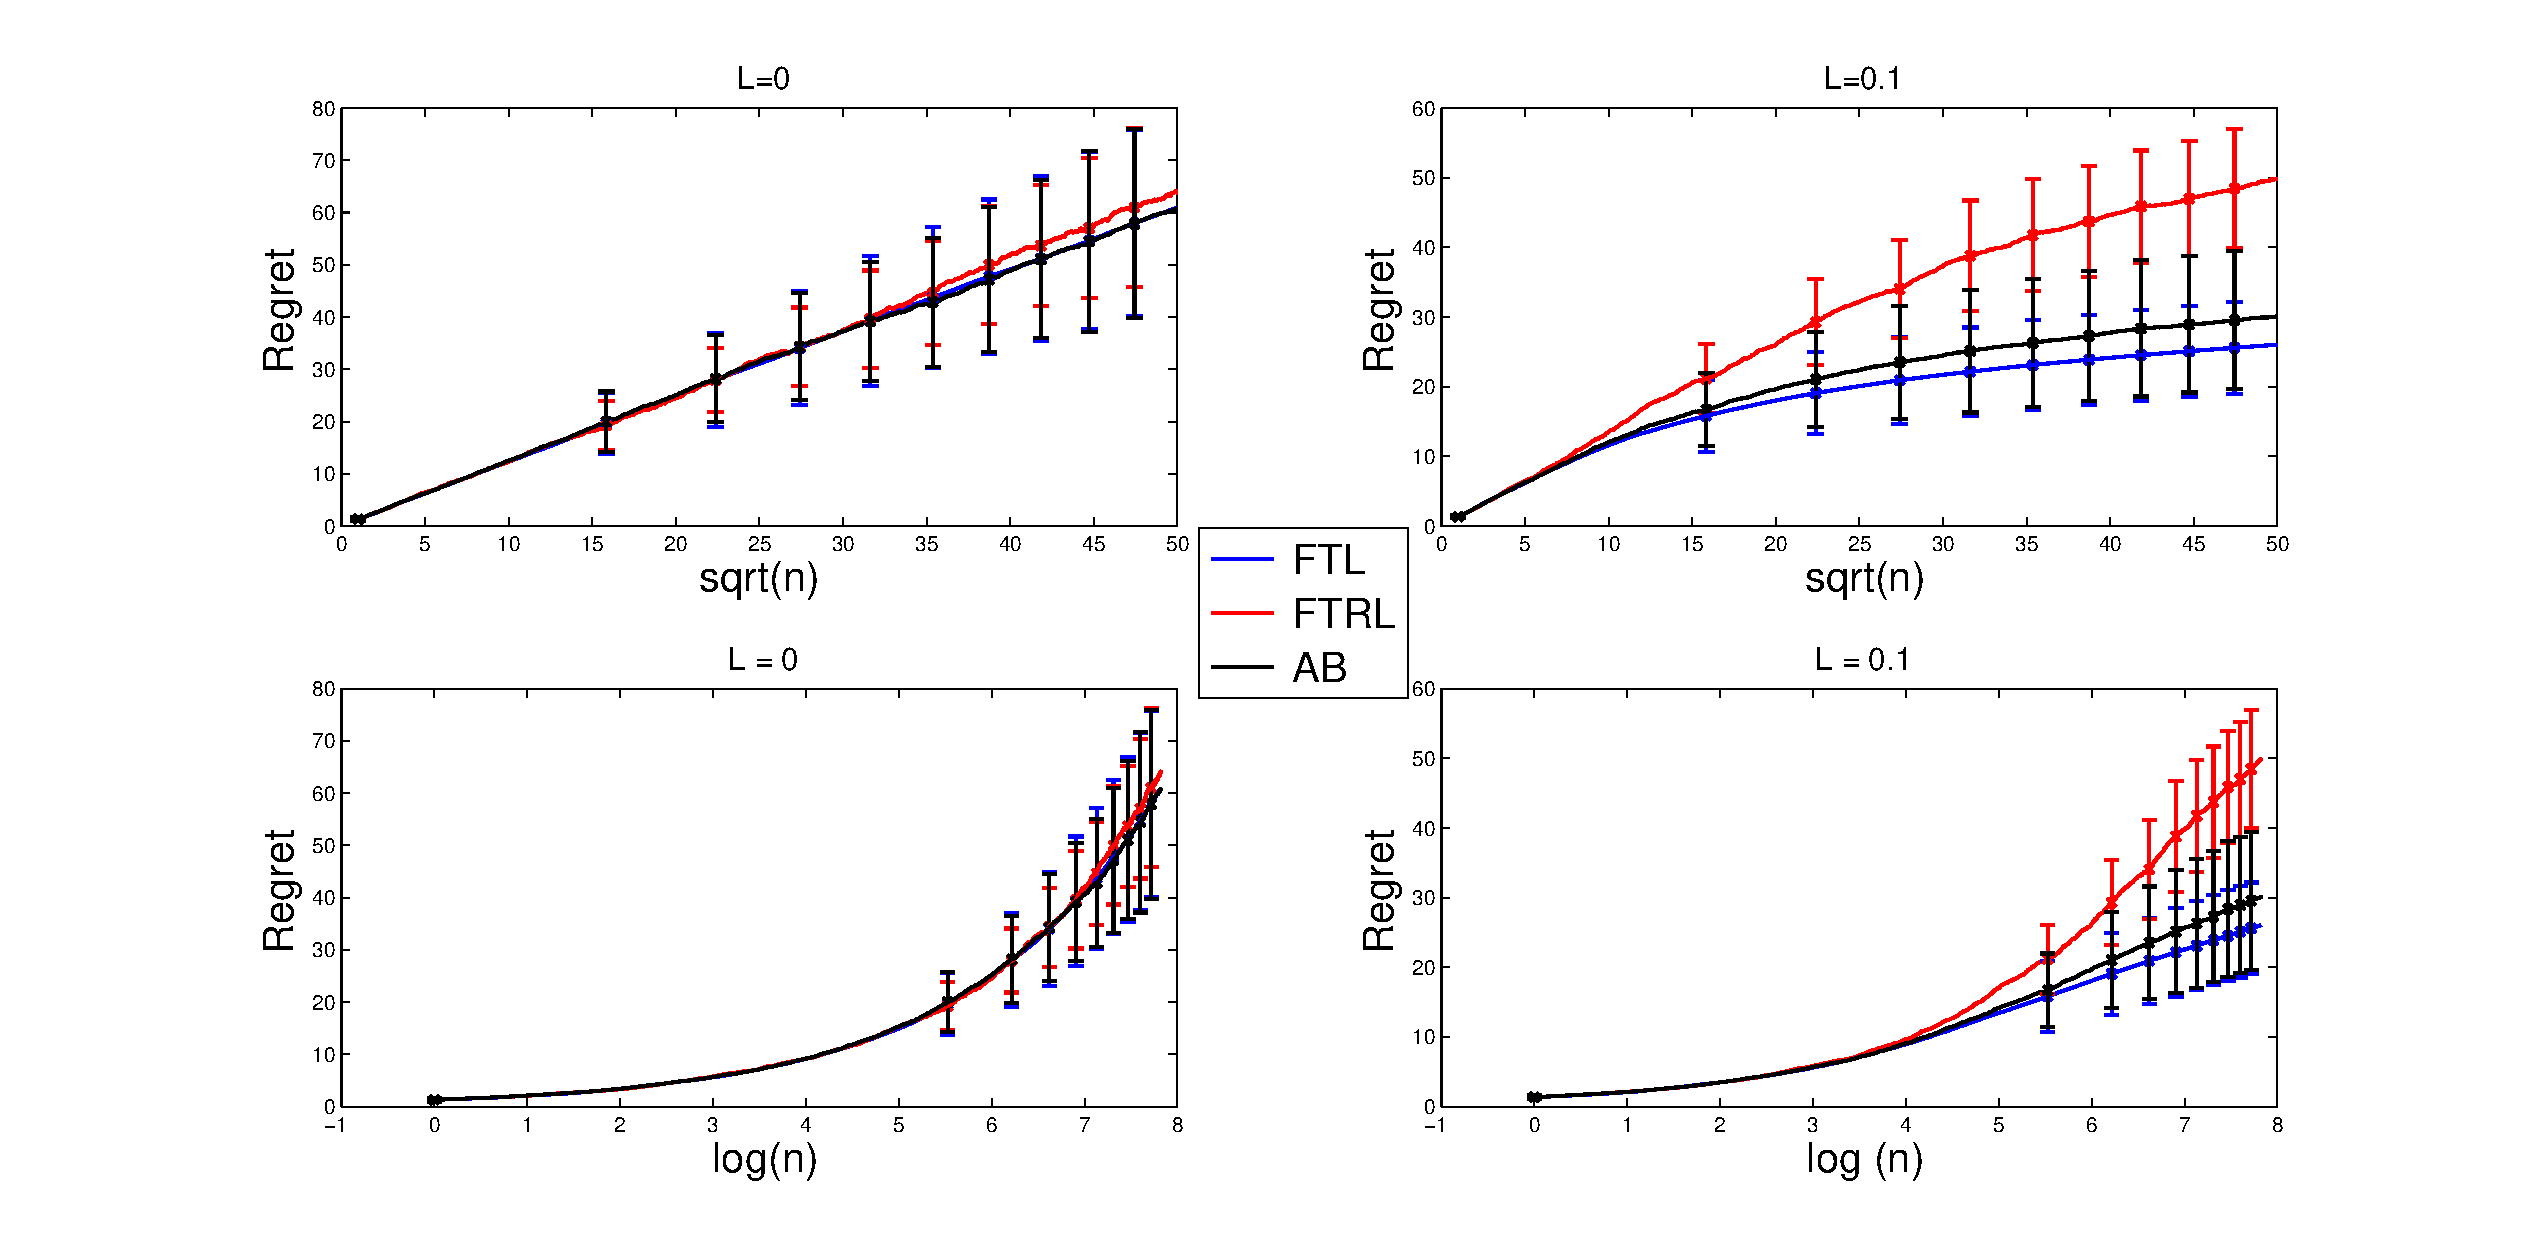
\includegraphics[height = 6cm]{figures/ExpResults/Stoc}
	
\footnotesize
\begin{itemize}
\item $\cW$: 4-dimensional ellipsoid centered at the origin
\item $f_t=L e_1 + \hf_t$ with $\hf_t$ uniformly distributed unit vector
\end{itemize}

\end{frame}

\begin{frame}{Experiments: "Half adversarial" data}
	\centering
	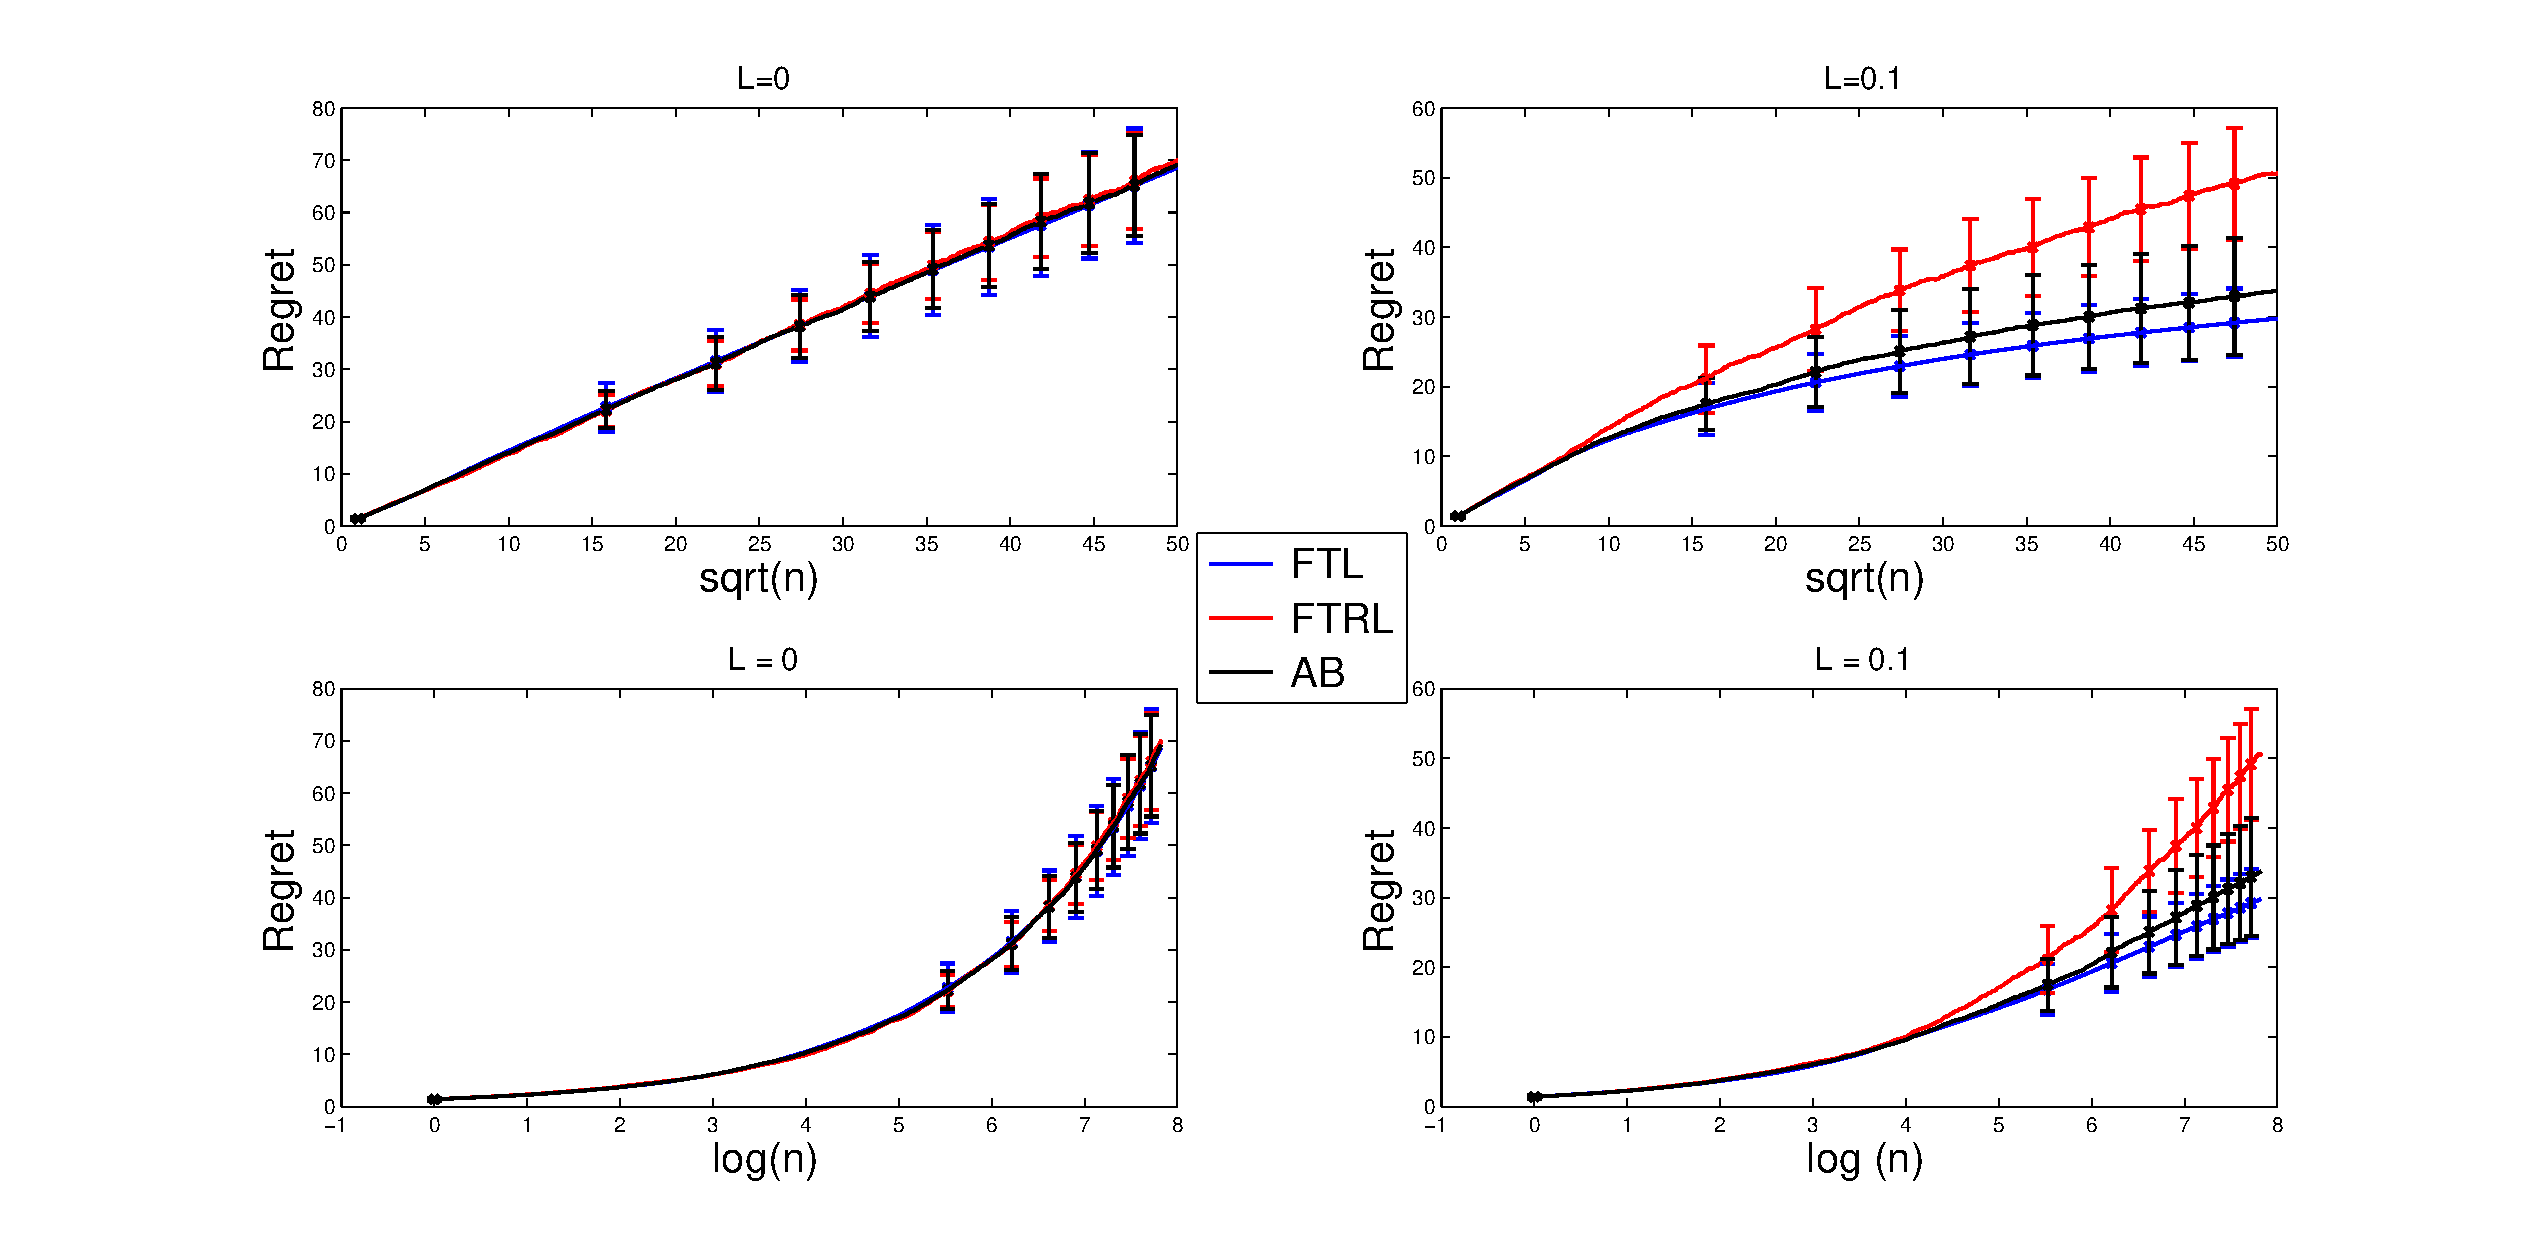
\includegraphics[height = 6cm]{figures/ExpResults/Adve}

\footnotesize
\begin{itemize}
\item $\hf_t$: $(d-1)$-dimensional unit vectors, orthogonal to $\sum_{i=1}^{t-1} \hf_i$, uniform distribution
\item $f_t=(L, \sqrt{1-L^2} \hf_t)$
\end{itemize}
\end{frame}

\begin{frame}{Experiments: Adversarial data}
	\centering
	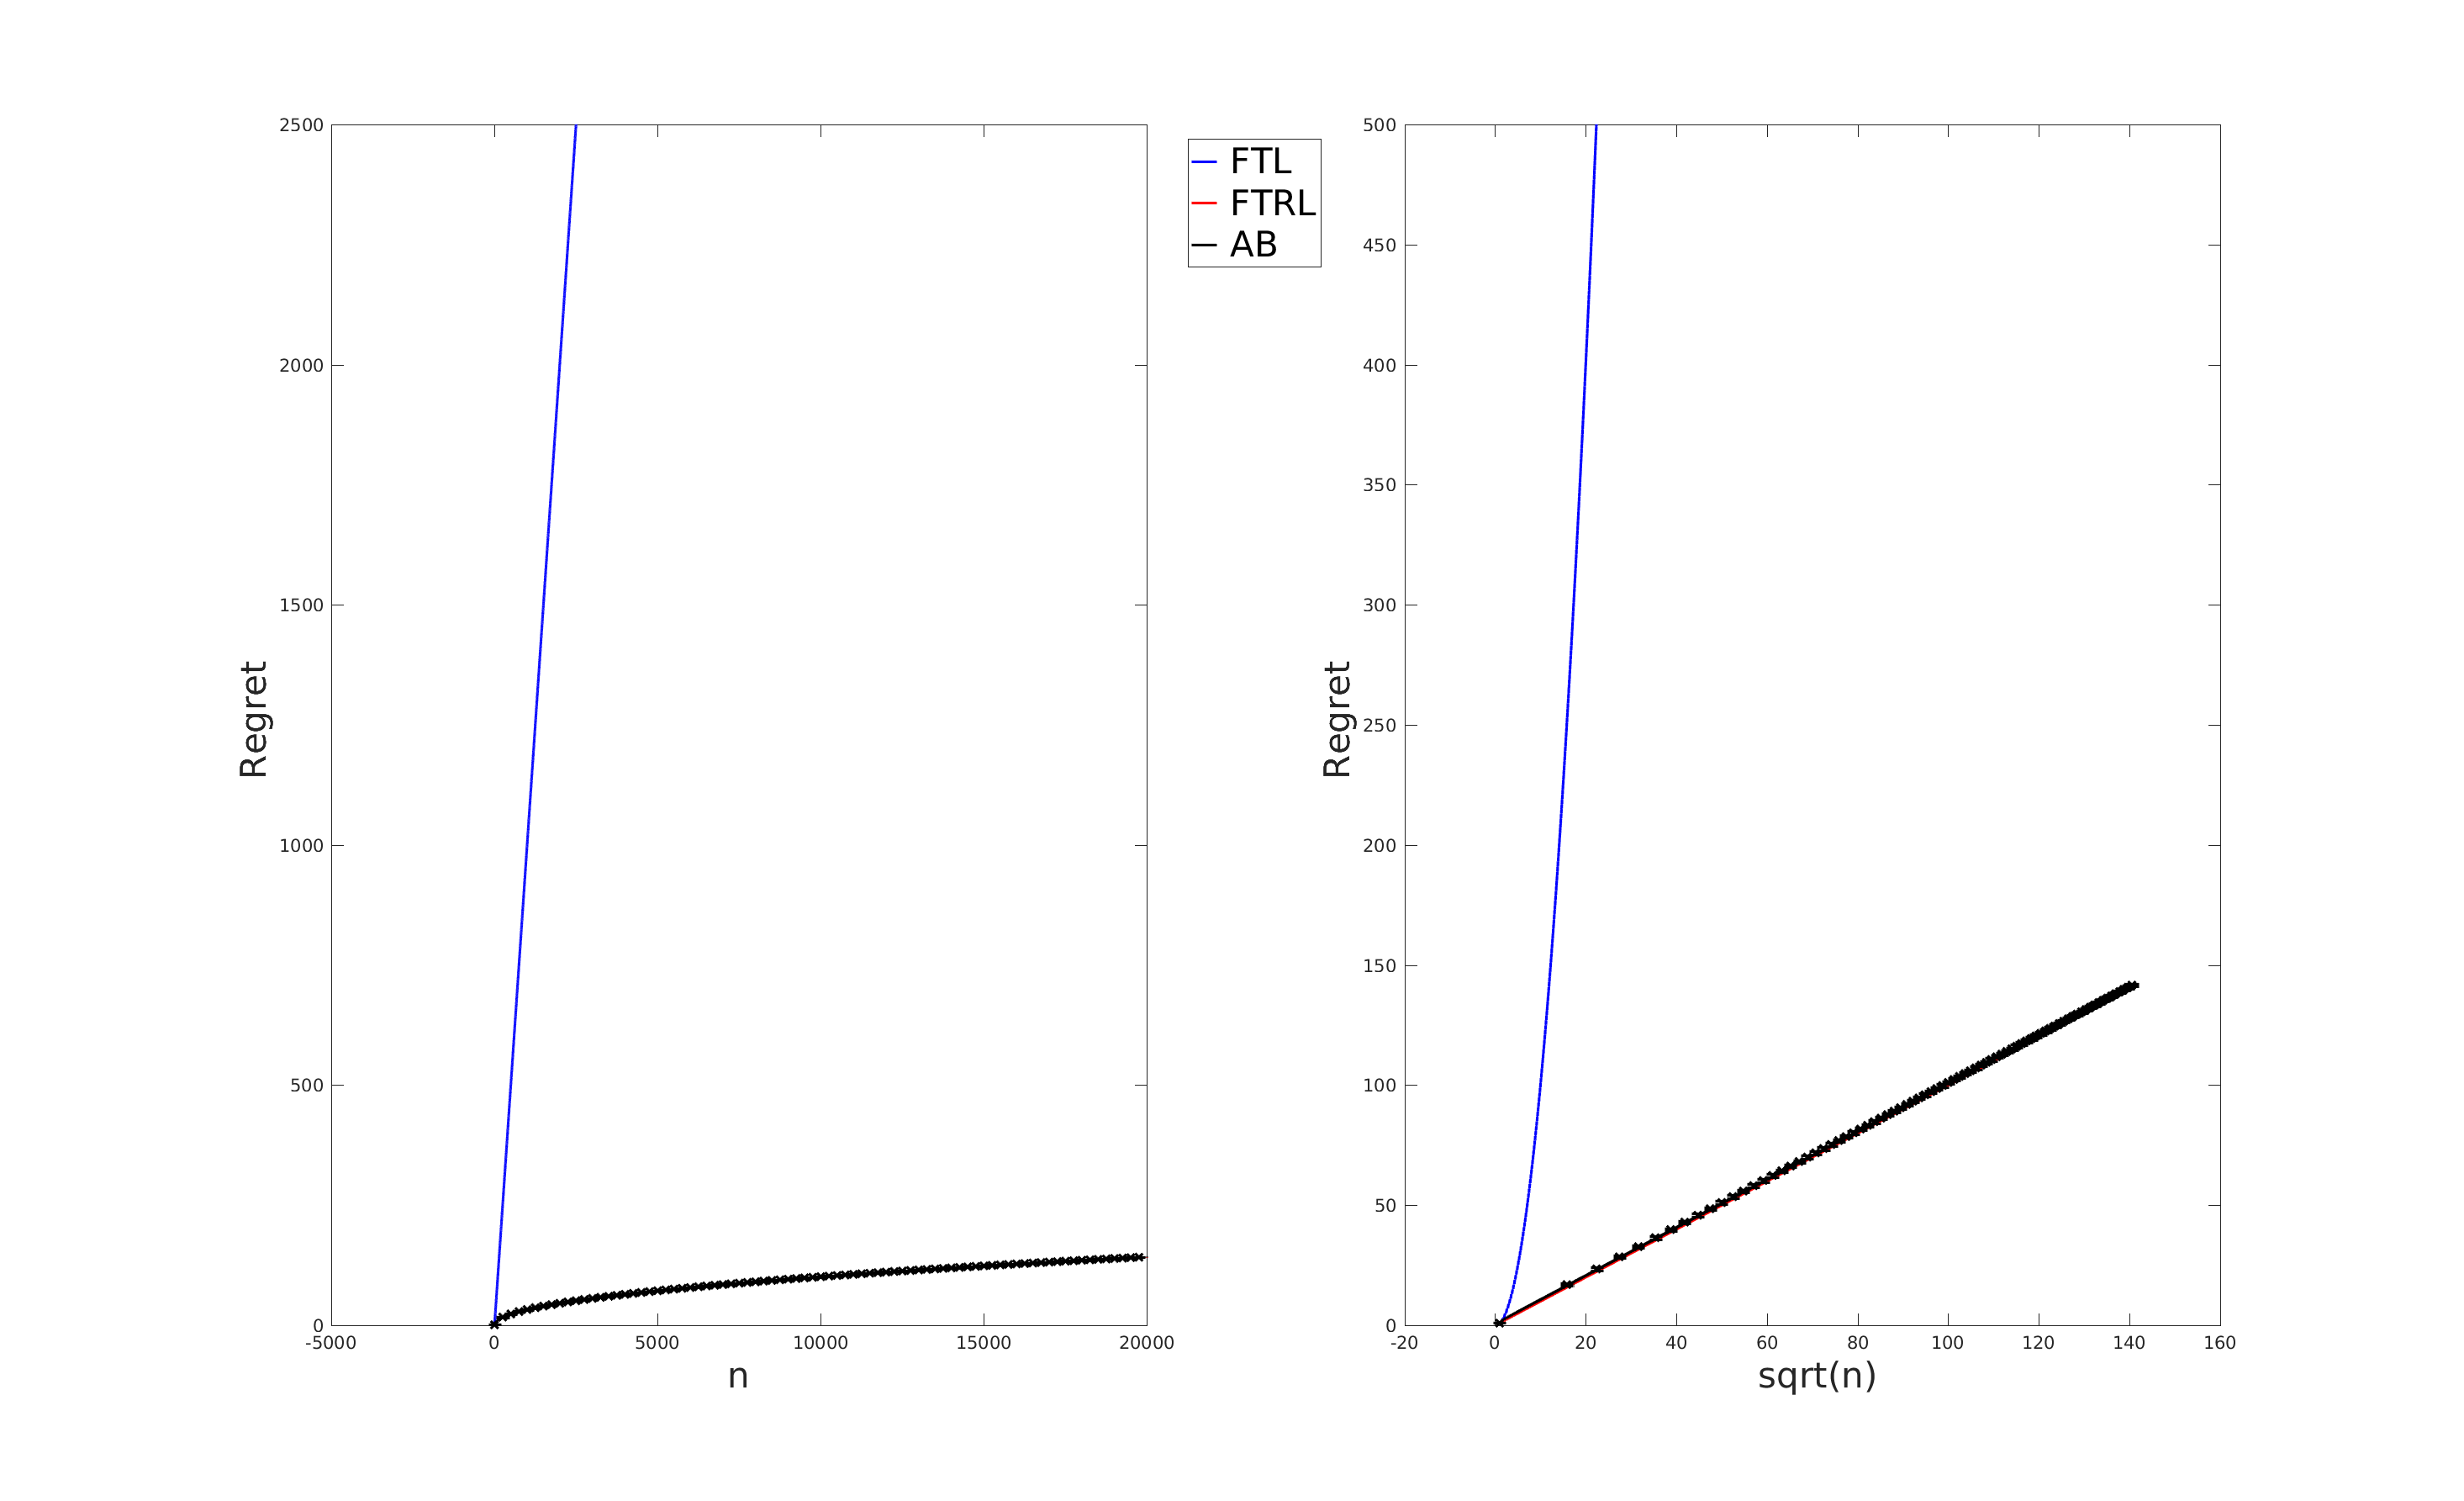
\includegraphics[height = 6cm]{figures/ExpResults/WorstCase_alt2}
\footnotesize
\begin{itemize}
\item $f_t=(\hf_t,0,\ldots,0)$
\item $(\hf_t)_t = 0.9, -1,1,-1,1,\ldots$
\end{itemize}
\end{frame}


\begin{frame}{Lessons learned for FTL}
\begin{itemize}
\item Shape of the constraint set may help \bigskip
\item Other algorithms? \bigskip
\item Generalization:  \bigskip
\begin{itemize}
\item Cheating algorithm: predict $w_{t+1}$ at time $t$ \medskip
\item Control $\ell_t(w_t)-\ell_t(w_{t-1})$ \medskip
\item What else can help? \medskip
\item Conjecture: $\ell_t$ $\alpha$-expconcave, minimum curvature $\lambda_0$ $\Rightarrow$ $O(\log(n)/(\alpha+\lambda_0))$ regret when the optimum is outside $\cW$
\end{itemize}
\end{itemize}
\end{frame}

\begin{frame}{Conclusion}
\linespread{1.5}
\bi
\item Understanding when and why certain learning algorithms work is crucial 
for closing the gap between theory and practice
\item Deterministic analysis could help
\bi
\item Cleaner, more general
\ei
\item Finding new regularities that make learning faster is important
\item The above ideas were demonstrated in two settings:
\bi
\item independent component analysis
\item follow-the-leader algorithm in online learning
\ei
\item Should be done more often!
\bi
\item Applicable to deep neural networks?
\ei
\ei
\end{frame}

%%%%%%%%%%%%%%%%%%%%%%%%%%%%%%%%%%%%%%%%
\section*{References}
%%%%%%%%%%%%%%%%%%%%%%%%%%%%%%%%%%%%%%%%

\begin{frame}[allowframebreaks]{References}
%\begin{frame}{References}
    \Fontvi
%	\scriptsize 
%	\begin{multicols}{2} % from \usepackage{multicol}
	\bibliography{reference,DICA}
	\bibliographystyle{plainnat}
%	\end{multicols}
\end{frame}
%%%%%%%%%%%%%%%%%%%%%%%%%%%%%%%%%%%%%%%%

\begin{frame}{Proof Sketch of the Adaptive Algorithm}
Idea from \citet{abernethy2008optimal}:
\begin{align*}
	V_n & = \max_{f_1, \ldots, f_n} \sum_{t=1}^{n}\inpro{w_t}{f_t}- \min_{w\in\cW} \inpro{w}{F_n} \\
	& \le \max_{f_1,\ldots, f_{n-1}} \sum_{t=1}^{n-1}\inpro{w_t}{f_t} + \sqrt{\|F_{n-1}\|_2^2 + n} \\
	& \le \max_{f_1,\ldots, f_{n-2}} \sum_{t=1}^{n-2}\inpro{w_t}{f_t}  + \sqrt{\|F_{n-2}\|_2^2 + n-1} + \frac{1}{\sqrt{n}} \\
& \le \ldots \\
& \le \sum_{t=1}^{n}\frac{1}{\sqrt{t}} = O(\sqrt{n}).
\end{align*}
Worst case choice of $f_t$ (to maximize the bound) is orthogonal to $F_{t-1}$.
\end{frame}

\begin{frame}{Proof Sketch}
If $\|\Theta_t\| \ge L$:
\begin{align*}
	V_n & = \max_{f_1, \ldots, f_n} \sum_{t=1}^{n}\inpro{w_t}{f_t}- \min_{w\in\cW} \inpro{w}{F_n} \\
	& \le \max_{f_1,\ldots, f_{n-1}} \sum_{t=1}^{n-1}\inpro{w_t}{f_t} + \sqrt{\|F_{n-1}\|_2^2 + n} \\
	& \le \max_{f_1,\ldots, f_{n-2}} \sum_{t=1}^{n-2}\inpro{w_t}{f_t}  + \sqrt{\|F_{n-2}\|_2^2 + n-1} + \frac{1}{(n-1)L} \\
& \le \ldots \\
& \le 1+\sum_{t=1}^{n-1}\frac{1}{tL} = O(\log{n}/L).
\end{align*}
	
\end{frame}


% All of the following is optional and typically not needed. 
%\appendix
%\section<presentation>*{\appendixname}
%\subsection<presentation>*{For Further Reading}
%
%\begin{frame}[allowframebreaks]
%  \frametitle<presentation>{For Further Reading}
%    
%  \begin{thebibliography}{10}
%    
%  \beamertemplatebookbibitems
%  % Start with overview books.
%
%  \bibitem{Author1990}
%    A.~Author.
%    \newblock {\em Handbook of Everything}.
%    \newblock Some Press, 1990.
% 
%    
%  \beamertemplatearticlebibitems
%  % Followed by interesting articles. Keep the list short. 
%
%  \bibitem{Someone2000}
%    S.~Someone.
%    \newblock On this and that.
%    \newblock {\em Journal of This and That}, 2(1):50--100,
%    2000.
%  \end{thebibliography}
%\end{frame}
%



\end{document}




